% !TeX spellcheck = russian-aot-ieyo
% Зачем: Определяет класс документа (То, как будет выглядеть документ)
% Примечание: параметр draft помечает строки, вышедшие за границы страницы, прямоугольником, в фильной версии его нужно удалить.
\documentclass[a4paper,14pt,russian,oneside,final]{extreport}

% Зачем: Настройка Times New Roman.
% Рекомендовано для Windows (нужен PSCyr, подробности см. в fonts_windows.tex)
% раскомментировать, чтобы использовать:
%% Зачем: Предоставляет проприетарный Times New Roman.
% ОБНОВЛЕНИЕ: лучше использовать scalable-cyrfonts-tex: меньше проблем с установкой
% Из руководства к PSCyr: "Во избежание проблем пакет PSCyr должен загружаться перед пакета-ми inputenc и babel".
% Примечание: Требует шаманства при установке, инструкция http://plumbum-blog.blogspot.com/2010/06/miktex-28-pscyr-04d.html
% http://blog.harrix.org/?p=444
\usepackage{pscyr}

% Зачем: Выбор внутренней TeX кодировки.
\usepackage[T2A]{fontenc}

% не забудьте закомментировать % Зачем: Выбор внутренней TeX кодировки.
\usepackage[T2A]{fontenc}

% Зачем: Предоставляет свободный Times New Roman.
% Шрифт идёт вместе с пакетом scalable-cyrfonts-tex в Ubuntu/Debian

% пакет scalable-cyrfonts-tex может конфликтовать с texlive-fonts-extra в Ubuntu
% решение: Для себя я решил эту проблему так: пересобрал пакет scalable-cyrfonts-tex, изменив его имя. Решение топорное, но работает. Желающие могут скачать мой пакет здесь:
% https://yadi.sk/d/GW2PhDgEcJH7m
% Установка:
% dpkg -i scalable-cyrfonts-tex-shurph_4.16_all.deb

\usefont{T2A}{ftm}{m}{sl}


% Рекомендовано для Linux (нужен scalable-cyrfonts-tex, подробности см. в fonts_linux.tex)
% раскомментировать, чтобы использовать:
% Зачем: Выбор внутренней TeX кодировки.
\usepackage[T2A]{fontenc}

% Зачем: Предоставляет свободный Times New Roman.
% Шрифт идёт вместе с пакетом scalable-cyrfonts-tex в Ubuntu/Debian

% пакет scalable-cyrfonts-tex может конфликтовать с texlive-fonts-extra в Ubuntu
% решение: Для себя я решил эту проблему так: пересобрал пакет scalable-cyrfonts-tex, изменив его имя. Решение топорное, но работает. Желающие могут скачать мой пакет здесь:
% https://yadi.sk/d/GW2PhDgEcJH7m
% Установка:
% dpkg -i scalable-cyrfonts-tex-shurph_4.16_all.deb

\usefont{T2A}{ftm}{m}{sl}
% не забудьте закомментировать % Зачем: Предоставляет проприетарный Times New Roman.
% ОБНОВЛЕНИЕ: лучше использовать scalable-cyrfonts-tex: меньше проблем с установкой
% Из руководства к PSCyr: "Во избежание проблем пакет PSCyr должен загружаться перед пакета-ми inputenc и babel".
% Примечание: Требует шаманства при установке, инструкция http://plumbum-blog.blogspot.com/2010/06/miktex-28-pscyr-04d.html
% http://blog.harrix.org/?p=444
\usepackage{pscyr}

% Зачем: Выбор внутренней TeX кодировки.
\usepackage[T2A]{fontenc}



% Зачем: Установка кодировки исходных файлов.
\usepackage[utf8]{inputenc}

% Зачем: Делает результирующий PDF "searchable and copyable".
\usepackage{cmap}

% Зачем: Чтобы можно было использовать русские буквы в формулах, но в случае использования предупреждать об этом.
\usepackage[warn]{mathtext}

% Зачем: Учет особенностей различных языков.
\usepackage[russian]{babel}

% Зачем: Добавляет поддержу дополнительных размеров текста 8pt, 9pt, 10pt, 11pt, 12pt, 14pt, 17pt, and 20pt.
% Почему: Пункт 2.1.1 Требований по оформлению пояснительной записки.
\usepackage{extsizes}


% Зачем: Длинна, пимерно соответвующая 5 символам
% Почему: Требования содержат странное требование про отсупы в 5 символов (для немоноширинного шрифта :| )
\newlength{\fivecharsapprox}
\setlength{\fivecharsapprox}{6ex}


% Зачем: Добавляет отступы для абзацев.
% Почему: Пункт 2.1.3 Требований по оформлению пояснительной записки.
\usepackage{indentfirst}
\setlength{\parindent}{\fivecharsapprox} % Примерно соответсвует 5 символам.


% Зачем: Настраивает отступы от границ страницы.
% Почему: Пункт 2.1.2 Требований по оформлению пояснительной записки.
\usepackage[left=3cm,top=2.0cm,right=1.5cm,bottom=2.7cm]{geometry}


% Зачем: Настраивает межстрочный интервал, для размещения 40 +/- 3 строки текста на странице.
% Почему: Пункт 2.1.1 Требований по оформлению пояснительной записки.
\usepackage[nodisplayskipstretch]{setspace} 
\setstretch{1.1}
%\onehalfspacing

% Зачем: Выбор шрифта по-умолчанию. 
% Почему: Пункт 2.1.1 Требований по оформлению пояснительной записки.
% Примечание: В требованиях не указан, какой именно шрифт использовать. По традиции используем TNR.
\renewcommand{\rmdefault}{ftm} % Times New Roman


% Зачем: Отключает использование изменяемых межсловных пробелов.
% Почему: Так не принято делать в текстах на русском языке.
\frenchspacing


% Зачем: Сброс счетчика сносок для каждой страницы
% Примечание: в "Требованиях по оформлению пояснительной записки" не указано, как нужно делать, но в других БГУИРовских докуметах рекомендуется нумерация отдельная для каждой страницы
\usepackage{perpage}
\MakePerPage{footnote}


% Зачем: Добавляет скобку 1) к номеру сноски
% Почему: Пункты 2.9.2 и 2.9.1 Требований по оформлению пояснительной записки.
\makeatletter 
\def\@makefnmark{\hbox{\@textsuperscript{\normalfont\@thefnmark)}}}
\makeatother


% Зачем: Расположение сносок внизу страницы
% Почему: Пункт 2.9.2 Требований по оформлению пояснительной записки.
\usepackage[bottom]{footmisc}


% Зачем: Переопределяем стандартную нумерацию, т.к. в отчете будут только section и т.д. в терминологии TeX
\makeatletter
\renewcommand{\thesection}{\arabic{section}}
\makeatother


% Зачем: Пункты (в терминологии требований) в терминологии TeX subsubsection должны нумероваться
% Почему: Пункт 2.2.3 Требований по оформлению пояснительной записки.
\setcounter{secnumdepth}{3}


% Зачем: Настраивает отступ между таблицей с содержанимем и словом СОДЕРЖАНИЕ
% Почему: Пункт 2.2.7 Требований по оформлению пояснительной записки.
\usepackage{tocloft}
\setlength{\cftbeforetoctitleskip}{-1em}
\setlength{\cftaftertoctitleskip}{1em}


% Зачем: Определяет отступы слева для записей в таблице содержания.
% Почему: Пункт 2.2.7 Требований по оформлению пояснительной записки.
\makeatletter
\renewcommand{\l@section}{\@dottedtocline{1}{0.5em}{1.2em}}
\renewcommand{\l@subsection}{\@dottedtocline{2}{1.7em}{2.0em}}
\makeatother


% Зачем: Работа с колонтитулами
\usepackage{fancyhdr} % пакет для установки колонтитулов
\pagestyle{fancy} % смена стиля оформления страниц


% Зачем: Нумерация страниц располагается справа снизу страницы
% Почему: Пункт 2.2.8 Требований по оформлению пояснительной записки.
\fancyhf{} % очистка текущих значений
\fancyfoot[R]{\thepage} % установка верхнего колонтитула
\renewcommand{\footrulewidth}{0pt} % убрать разделительную линию внизу страницы
\renewcommand{\headrulewidth}{0pt} % убрать разделительную линию вверху страницы
\fancypagestyle{plain}{ 
    \fancyhf{}
    \rfoot{\thepage}}


% Зачем: Задает стиль заголовков раздела жирным шрифтом, прописными буквами, без точки в конце
% Почему: Пункты 2.1.1, 2.2.5, 2.2.6 и ПРИЛОЖЕНИЕ Л Требований по оформлению пояснительной записки.
\makeatletter
\renewcommand\section{%
  \clearpage\@startsection {section}{1}%
    {\fivecharsapprox}%
    {-1em \@plus -1ex \@minus -.2ex}%
    {1em \@plus .2ex}%
    {\raggedright\hyphenpenalty=10000\normalfont\large\bfseries\MakeUppercase}}
\makeatother


% Зачем: Задает стиль заголовков подразделов
% Почему: Пункты 2.1.1, 2.2.5 и ПРИЛОЖЕНИЕ Л Требований по оформлению пояснительной записки.
\makeatletter
\renewcommand\subsection{%
  \@startsection{subsection}{2}%
    {\fivecharsapprox}%
    {-1em \@plus -1ex \@minus -.2ex}%
    {1em \@plus .2ex}%
    {\raggedright\hyphenpenalty=10000\normalfont\normalsize\bfseries}}
\makeatother


% Зачем: Задает стиль заголовков пунктов
% Почему: Пункты 2.1.1, 2.2.5 и ПРИЛОЖЕНИЕ Л Требований по оформлению пояснительной записки.
\makeatletter
\renewcommand\subsubsection{
  \@startsection{subsubsection}{3}%
    {\fivecharsapprox}%
    {-1em \@plus -1ex \@minus -.2ex}%
    {\z@}%
    {\raggedright\hyphenpenalty=10000\normalfont\normalsize\bfseries}}
\makeatother

% Зачем: для оформления введения и заключения, они должны быть выровнены по центру.
% Почему: Пункты 1.1.15 и 1.1.11 Требований по оформлению пояснительной записки.
\makeatletter
\newcommand\sectioncentered{%
  \clearpage\@startsection {section}{1}%
    {\z@}%
    {-1em \@plus -1ex \@minus -.2ex}%
    {1em \@plus .2ex}%
    {\centering\hyphenpenalty=10000\normalfont\large\bfseries\MakeUppercase}%
    }
\makeatother



% Зачем: Задает стиль библиографии
% Почему: Пункт 2.8.6 Требований по оформлению пояснительной записки.
\bibliographystyle{styles/belarus-specific-utf8gost780u}


% Зачем: Пакет для вставки картинок
% Примечание: Объяснение, зачем final - http://tex.stackexchange.com/questions/11004/why-does-the-image-not-appear
\usepackage[final]{graphicx}
\DeclareGraphicsExtensions{.pdf,.png,.jpg,.eps}


% Зачем: Директория в которой будет происходить поиск картинок
\graphicspath{{figures/}}


% Зачем: Добавление подписей к рисункам
\usepackage[nooneline]{caption}
\usepackage{subcaption}

% Зачем: чтобы работала \No в новых латехах
\DeclareRobustCommand{\No}{\ifmmode{\nfss@text{\textnumero}}\else\textnumero\fi}

% Зачем: поворот ячеек таблиц на 90 градусов
\usepackage{rotating}
\DeclareRobustCommand{\povernut}[1]{\begin{sideways}{#1}\end{sideways}}


% Зачем: когда в формулах много кириллических символов команда \text{} занимает много места
\DeclareRobustCommand{\x}[1]{\text{#1}}


% Зачем: Задание подписей, разделителя и нумерации частей рисунков
% Почему: Пункт 2.5.5 Требований по оформлению пояснительной записки.
\DeclareCaptionLabelFormat{stbfigure}{Рисунок #2}
\DeclareCaptionLabelFormat{stbtable}{Таблица #2}
\DeclareCaptionLabelSeparator{stb}{~--~}
\captionsetup{labelsep=stb}
\captionsetup[figure]{labelformat=stbfigure,justification=centering}
\captionsetup[table]{labelformat=stbtable,justification=raggedright}
\renewcommand{\thesubfigure}{\asbuk{subfigure}}

% Зачем: Окружения для оформления формул
% Почему: Пункт 2.4.7 требований по оформлению пояснительной записки и специфические требования различных кафедр
% Пример использования смотри в course_content.tex, строка 5
\usepackage{calc}
\newlength{\lengthWordWhere}
\settowidth{\lengthWordWhere}{где}
\newenvironment{explanationx}
    {%
    %%% Следующие строки определяют специфические требования разных редакций стандартов. Раскоменнтируйте нужную строку
    %% стандартный абзац, СТП-01 2010
    %\begin{itemize}[leftmargin=0cm, itemindent=\parindent + \lengthWordWhere + \labelsep, labelsep=\labelsep]
    %% без отступа, СТП-01 2013
    \begin{itemize}[leftmargin=0cm, itemindent=\lengthWordWhere + \labelsep , labelsep=\labelsep]%
    \renewcommand\labelitemi{}%
    }
    {%
    %\\[\parsep]
    \end{itemize}
    }

% Старое окружение для "где". Сохранено для совместимости
\usepackage{tabularx}

\newenvironment{explanation}
    {
    %%% Следующие строки определяют специфические требования разных редакций стандартов. Раскоменнтируйте нужные 2 строки
    %% стандартный абзац, СТП-01 2010
    %\par 
    %\tabularx{\textwidth-\fivecharsapprox}{@{}ll@{ --- } X }
    %% без отступа, СТП-01 2013
    \noindent 
    \tabularx{\textwidth}{@{}ll@{ --- } X }
    }
    { 
    \\[\parsep]
    \endtabularx
    }


% Зачем: Удобная вёрстка многострочных формул, масштабирующийся текст в формулах, формулы в рамках и др
\usepackage{amsmath}


% Зачем: Поддержка ажурного и готического шрифтов 
\usepackage{amsfonts}


% Зачем: amsfonts + несколько сотен дополнительных математических символов
\usepackage{amssymb}


% Зачем: Окружения «теорема», «лемма»
\usepackage{amsthm}


% Зачем: Производить арифметические операции во время компиляции TeX файла
\usepackage{calc}

% Зачем: Производить арифметические операции во время компиляции TeX файла
\usepackage{fp}

% Зачем: Пакет для работы с перечислениями
\usepackage{enumitem}
\makeatletter
 \AddEnumerateCounter{\asbuk}{\@asbuk}{щ)}
\makeatother


% Зачем: Устанавливает символ начала простого перечисления
% Почему: Пункт 2.3.5 Требований по оформлению пояснительной записки.
\setlist{nolistsep}


% Зачем: Устанавливает символ начала именованного перечисления
% Почему: Пункт 2.3.8 Требований по оформлению пояснительной записки.
\renewcommand{\labelenumi}{\asbuk{enumi})}
\renewcommand{\labelenumii}{\arabic{enumii})}

% Зачем: Устанавливает отступ от границы документа до символа списка, чтобы этот отступ равнялся отступу параграфа
% Почему: Пункт 2.3.5 Требований по оформлению пояснительной записки.

\setlist[itemize,0]{itemindent=\parindent + 2.2ex,leftmargin=0ex,label=--}
\setlist[enumerate,1]{itemindent=\parindent + 2.7ex,leftmargin=0ex}
\setlist[enumerate,2]{itemindent=\parindent + \parindent - 2.7ex}

% Зачем: Включение номера раздела в номер формулы. Нумерация формул внутри раздела.
\AtBeginDocument{\numberwithin{equation}{section}}

% Зачем: Включение номера раздела в номер таблицы. Нумерация таблиц внутри раздела.
\AtBeginDocument{\numberwithin{table}{section}}

% Зачем: Включение номера раздела в номер рисунка. Нумерация рисунков внутри раздела.
\AtBeginDocument{\numberwithin{figure}{section}}


% Зачем: Дополнительные возможности в форматировании таблиц
\usepackage{makecell}
\usepackage{multirow}
\usepackage{array}


% Зачем: "Умная" запятая в математических формулах. В дробных числах не добавляет пробел
% Почему: В требованиях не нашел, но в русском языке для дробных чисел используется {,} а не {.}
\usepackage{icomma}

% Зачем: макрос для печати римских чисел
\makeatletter
\newcommand{\rmnum}[1]{\romannumeral #1}
\newcommand{\Rmnum}[1]{\expandafter\@slowromancap\romannumeral #1@}
\makeatother


% Зачем: Управление выводом чисел.
\usepackage{sistyle}
\SIdecimalsign{,}

% Зачем: inline-коментирование содержимого.
\newcommand{\ignore}[2]{\hspace{0in}#2}


% Зачем: Возможность коментировать большие участки документа
\usepackage{verbatim}


\usepackage{xcolor}


% Зачем: Оформление листингов кода
% Примечание: final нужен для переопределения режима draft, в котором листинги не выводятся в документ.
\usepackage[final]{listings}


% Зачем: настройка оформления листинга для языка F#
\definecolor{bluekeywords}{rgb}{0.13,0.13,1}
\definecolor{greencomments}{rgb}{0,0.5,0}
\definecolor{turqusnumbers}{rgb}{0.17,0.57,0.69}
\definecolor{redstrings}{rgb}{0.5,0,0}

\renewcommand{\lstlistingname}{Листинг}

\lstdefinelanguage{FSharp}
    {morekeywords={abstract,and,as,assert,base,begin,class,default,delegate,do,done,downcast,downto,elif,else,end,exception,extern,false,finally,for,fun,function,global,if,in,inherit,inline,interface,internal,lazy,let,let!,match,member,module,mutable,namespace,new,not,null,of,open,or,override,private,public,rec,return,return!,select,static,struct,then,to,true,try,type,upcast,use,use!,val,void,when,while,with,yield,yield!,asr,land,lor,lsl,lsr,lxor,mod,sig,atomic,break,checked,component,const,constraint,constructor,continue,eager,event,external,fixed,functor,include,method,mixin,object,parallel,process,protected,pure,sealed,tailcall,trait,virtual,volatile},
    keywordstyle=\bfseries\color{bluekeywords},
    sensitive=false,
    morecomment=[l][\color{greencomments}]{///},
    morecomment=[l][\color{greencomments}]{//},
    morecomment=[s][\color{greencomments}]{{(*}{*)}},
    morestring=[b]",
    stringstyle=\color{redstrings},
    }

\lstdefinestyle{fsharpstyle}{
   xleftmargin=0ex,
   language=FSharp,
   basicstyle=\footnotesize\ttfamily,
   breaklines=true,
   columns=fullflexible
}

\lstdefinestyle{csharpinlinestyle} {
  language=[Sharp]C,
  morekeywords={yield,var,get,set,from,select,partial,where,async,await},
  breaklines=true,
  columns=fullflexible,
  basicstyle=\footnotesize\ttfamily
}

\lstdefinestyle{csharpstyle}{
  language=[Sharp]C,
  frame=lr,
  rulecolor=\color{blue!80!black}}


% Зачем: Нумерация листингов в пределах секции
\AtBeginDocument{\numberwithin{lstlisting}{section}}

\usepackage[normalem]{ulem}

\usepackage[final,hidelinks]{hyperref}
% Моноширинный шрифт выглядит визуально больше, чем пропорциональный шрифт, если их размеры одинаковы. Искусственно уменьшаем размер ссылок.
\renewcommand{\UrlFont}{\small\rmfamily\tt}

\usepackage[square,numbers,sort&compress]{natbib}
\setlength{\bibsep}{0em}

% Магия для подсчета разнообразных объектов в документе
\usepackage{lastpage}
\usepackage{totcount}
\regtotcounter{section}

\usepackage{etoolbox}

\newcounter{totfigures}
\newcounter{tottables}
\newcounter{totreferences}
\newcounter{totequation}

\providecommand\totfig{} 
\providecommand\tottab{}
\providecommand\totref{}
\providecommand\toteq{}

\makeatletter
\AtEndDocument{%
  \addtocounter{totfigures}{\value{figure}}%
  \addtocounter{tottables}{\value{table}}%
  \addtocounter{totequation}{\value{equation}}
  \immediate\write\@mainaux{%
    \string\gdef\string\totfig{\number\value{totfigures}}%
    \string\gdef\string\tottab{\number\value{tottables}}%
    \string\gdef\string\totref{\number\value{totreferences}}%
    \string\gdef\string\toteq{\number\value{totequation}}%
  }%
}
\makeatother

\pretocmd{\section}{\addtocounter{totfigures}{\value{figure}}\setcounter{figure}{0}}{}{}
\pretocmd{\section}{\addtocounter{tottables}{\value{table}}\setcounter{table}{0}}{}{}
\pretocmd{\section}{\addtocounter{totequation}{\value{equation}}\setcounter{equation}{0}}{}{}
\pretocmd{\bibitem}{\addtocounter{totreferences}{1}}{}{}



% Для оформления таблиц не влязящих на 1 страницу
\usepackage{longtable}

% Для включения pdf документов в результирующий файл
\usepackage{pdfpages}

% Для использования знака градуса и других знаков
% http://ctan.org/pkg/gensymb
\usepackage{gensymb}

% Зачем: преобразовывать текст в верхний регистр командой MakeTextUppercase
\usepackage{textcase}

% Зачем: Переносы в словах с тире.
% Тире в словае заменяем на \hyph: аппаратно\hyphпрограммный.
% https://stackoverflow.com/questions/2193307/how-to-get-latex-to-hyphenate-a-word-that-contains-a-dash#
\def\hyph{-\penalty0\hskip0pt\relax}

% Добавляем абзацный отступ для библиографии
% https://github.com/mstyura/bsuir-diploma-latex/issues/19
\setlength\bibindent{-1.0900cm}

\makeatletter
\renewcommand\NAT@bibsetnum[1]{\settowidth\labelwidth{\@biblabel{#1}}%
   \setlength{\leftmargin}{\bibindent}\addtolength{\leftmargin}{\dimexpr\labelwidth+\labelsep\relax}%
   \setlength{\itemindent}{-\bibindent+\fivecharsapprox-0.240cm}%
   \setlength{\listparindent}{\itemindent}
\setlength{\itemsep}{\bibsep}\setlength{\parsep}{\z@}%
   \ifNAT@openbib
     \addtolength{\leftmargin}{\bibindent}%
     \setlength{\itemindent}{-\bibindent}%
     \setlength{\listparindent}{\itemindent}%
     \setlength{\parsep}{10pt}%
   \fi
}



\newcommand{\csharp}{C\#}
\newcommand{\fsharp}{F\#}
\newcommand{\vbnet}{Visual Basic~.NET}
\newcommand{\cpp}{C\texttt{\hspace{-0.3ex}+\hspace{-0.25ex}+}}
\newcommand{\cppcli}{Visual \cpp{}/CLI}
\newcommand{\dotnet}{Microsoft .NET}
\newcommand{\netfx}{.NET Framework}
\newcommand{\java}{Java}

\begin{document}

\begin{titlepage}
  \begin{center}
    Министерство образования Республики Беларусь\\[1em]
    Учреждение образования\\
    БЕЛОРУССКИЙ ГОСУДАРСТВЕННЫЙ УНИВЕРСИТЕТ \\
    ИНФОРМАТИКИ И РАДИОЭЛЕКТРОНИКИ\\[1em]

    \begin{minipage}{\textwidth}
      \begin{flushleft}
        \begin{tabular}{ l l }
          Факультет & Компьютерных систем и сетей\\
          Кафедра   & Информатики
        \end{tabular}
      \end{flushleft}
    \end{minipage}\\[1em]

    \begin{flushright}
      \begin{minipage}{0.4\textwidth}
        \textit{К защите допустить:}\\[0.8em]
        Заведующий кафедрой ИИтП\\[0.45em]
        \underline{\hspace*{2.8cm}} Н.\,А.~Волорова
      \end{minipage}\\[2.2em]
    \end{flushright}

    %%
    %% ВНИМАНИЕ: на некторых факультетах (ФКП) и кафедрах (ПИКС) слова "ПОЯСНИТЕЛЬНАЯ ЗАПИСКА" предлагается (требуется) оформлять полужирным начертанием. Раскомментируйте нужную для вас строку:
    %%
    %\textbf{ПОЯСНИТЕЛЬНАЯ ЗАПИСКА}\\
    {ПОЯСНИТЕЛЬНАЯ ЗАПИСКА}\\
    {к дипломному проекту}\\
    {на тему:}\\[1em]
    \textbf{\large Языковая модель дл белорусского языка на основе нейронных сетей}\\[1em]


    {БГУИР ДП Какие-то циферки}\\[2em]
    
    \begin{tabular}{ p{0.65\textwidth}p{0.25\textwidth} }
      Студент & А.\,Б.~Яковлев \\
      Руководитель & М.\,А.~Калугина \\
      Консультанты: &\\
      \hspace*{3ex}\emph{от кафедры информатики} & А.\,А.~Калугина \\
      \hspace*{3ex}\emph{по экономической части} & С.\,В.~Наркевич \\
      %%
      %% ВНИМАНИЕ: в зависимости от выбранной темы, у вас консультант может быть как по охране труда, так и по:
        % экологической безопасности
        % ресурсосбережению
        % энергосбережению
      %%
      %% Впишите правильную формулировку по необходимости
      %\hspace*{3ex}\emph{по охране труда} & Е.\,А.~Колосова \\
      Нормоконтролёр & В.\,В.~Шиманский\\
      & \\
      Рецензент &
    \end{tabular}
    
    \vfill
    {\normalsize Минск 2022}
  \end{center}
\end{titlepage}
 % page 1

%\sectioncentered*{Реферат}
\thispagestyle{empty}
%%
%% ВНИМАНИЕ: этот реферат не соответствует СТП-01 2013
%% пример оформления реферата смотрите здесь: http://www.bsuir.by/m/12_100229_1_91132.docx 
%%

\emph{Ключевые слова}: вероятностные модели; байесовы сети; вывод структуры сети по данным; принцип минимальной длинны описания; оценка апостериорной вероятности.

\vspace{4\parsep}

Дипломный проект выполнен на 6 листах формата А1 с пояснительной запиской на~\pageref*{LastPage} страницах, без приложений справочного или информационного характера. 
Пояснительная записка включает \total{section}~глав, \totfig{}~рисунков, \tottab{}~таблиц, \toteq{}~формул и \totref{}~литературный источник.

Целью дипломного проекта является разработка удобного в использовании инструмента, пригодного для решения практических задач, возникающих в реальных проектах, связанных с вероятностным моделированием.

Для достижения цели дипломного проекта была разработана библиотека кода для \dotnet{}, предназначенная для представления и обучения структуры вероятностной сети по экспериментальным данным.
Библиотека может быть использована в реальных проектах, использующих вероятностный подход к решению проблемы.
В библиотеке реализовано несколько алгоритмов, имеющих различные качественные характеристики.

В разделе технико"=экономического обоснования был произведён расчёт затрат на создание ПО, а также прибыли от разработки, получаемой разработчиком.
Проведённые расчёты показали экономическую целесообразность проекта.

Пояснительная записка включает раздел по охране труда, в котором была произведена оценка пожарной безопасности на предприятии, где частично разрабатывался данный дипломный проект.

\clearpage
 % page 2

%{
  \newgeometry{top=1.25cm,bottom=1.25cm,right=1cm,left=2cm,twoside}
  \thispagestyle{empty}
  \setlength{\parindent}{0em}

  \newcommand{\lineunderscore}{\uline{\hspace*{\fill}}}

  \begin{center}
    Министерство образования Республики Беларусь\\
    Учреждение образования\\
    БЕЛОРУССКИЙ ГОСУДАРСТВЕННЫЙ УНИВЕРСИТЕТ \\
    ИНФОРМАТИКИ И РАДИОЭЛЕКТРОНИКИ\\[1em]
  

  \begin{minipage}{\textwidth}
    \begin{flushleft}
      \begin{tabular}{ p{0.20\textwidth}p{0.31\textwidth}p{0.20\textwidth}p{0.20\textwidth} @{} }
        Факультет & КСиС & Кафедра & Информатики \\
        Специальность   & 1-31 03 04 & Специализация & 07
      \end{tabular}
    \end{flushleft}
  \end{minipage}\\[1em]

  \begin{minipage}{\textwidth}
    \begin{flushright}
      \begin{tabular}{p{0.40\textwidth}}
        УТВЕРЖДАЮ \\[0.5em]
        \underline{\hspace*{7em}} Зав. кафедрой \\
        <<\underline{\hspace*{4ex}}>> \underline{\hspace*{7em}} 2013 г.
      \end{tabular}
    \end{flushright}
  \end{minipage}\\[1em]

  \textbf{ЗАДАНИЕ} \\
  \textbf{по дипломному проекту (работе) студента}

  \lineunderscore \\
  {\small (фамилия, имя, отчество) }

  \end{center}

  1. Тема проекта (работы):
  \lineunderscore\\
  \lineunderscore\\
  \lineunderscore\\
  утверждена приказом по университету от \uline{\hspace*{1.5em}} \uline{\hspace*{5em}} 2013 г.  \No{} \uline{\hspace*{2em}}-с

  \vspace{1em}

  2. Срок сдачи студентом законченного проекта (работы): \lineunderscore

  \vspace{1em}

  3. Исходные данные к проекту (работе):
  \lineunderscore\\
  \lineunderscore\\
  \lineunderscore\\
  \lineunderscore\\
  \lineunderscore\\
  \lineunderscore

  \vspace{1em}

  4. Содержание пояснительной записки (перечень подлежащих разработке вопросов):
  \lineunderscore\\
  \lineunderscore\\
  \lineunderscore\\
  \lineunderscore\\
  \lineunderscore\\
  \lineunderscore\\
  \lineunderscore\\
  \lineunderscore\\
  \lineunderscore\\
  \lineunderscore\\
  \lineunderscore

  \clearpage
  \thispagestyle{empty}

  5. Перечень графического материала (с точным указанием обязательных чертежей):
  \lineunderscore\\
  \lineunderscore\\
  \lineunderscore\\
  \lineunderscore\\
  \lineunderscore\\
  \lineunderscore\\
  \lineunderscore\\
  \lineunderscore

  \vspace{1em}

  6. Содержание задания по технико-экономическому обоснованию:
  \lineunderscore\\
  \lineunderscore\\
  \lineunderscore

  Задание выдал: \hfill{} \uline{\hspace*{6em}} / И.\,О.~Фамилия /   

  \vspace{1em}

  7. Содержание задания по охране труда и экологической безопасности, ресурсо- и энергосбережению (\textit{указывается конкретное наименование раздела}): 
  \lineunderscore\\
  \lineunderscore\\
  \lineunderscore

  Задание выдал:  \hfill{} \uline{\hspace*{6em}} / И.\,О.~Фамилия /  

  \vfill

  \begin{center}
    КАЛЕНДАРНЫЙ ПЛАН
  \end{center}

  \begin{tabular}{| >{\centering}m{0.04\textwidth} 
                  | >{\centering}m{0.40\textwidth} 
                  | >{\centering}m{0.08\textwidth}
                  | >{\centering}m{0.19\textwidth}  
                  | >{\centering\arraybackslash}m{0.16\textwidth}|}
    \hline \No{} \No{} п/п & Наименование этапов дипломного проекта (работы) & Объем этапа, \% & Срок выполнения этапов & Примечание \\
    \hline & & & & \\
    \hline & & & & \\
    \hline & & & & \\
    \hline & & & & \\
    \hline & & & & \\
    \hline & & & & \\
    \hline & & & & \\
    \hline & & & & \\
    \hline & & & & \\
    \hline & & & & \\
    \hline & & & & \\
    \hline
  \end{tabular}

  \vspace{2em}

  Дата выдачи задания: \uline{\hspace*{6em}} \hspace{2ex} Руководитель \hfill{} \uline{\hspace*{4em}} / И.\,О.~Фамилия /

  \vspace{1em}

  Задание принял к исполнению \hfill{} \uline{\hspace*{4em}} / И.\,О.~Фамилия /

  \restoregeometry
} % pages 3 and 4. printed separately

%\sectioncentered*{Аннотация}
\thispagestyle{empty}

\begin{center}
  \begin{minipage}{0.82\textwidth}
    на дипломный проект <<Алгоритмы построения вероятностных сетей>> студента УО <<Белорусский государственный университет информатики и радиоэлектроники>> Ярошевича~Ю.\,А.
  \end{minipage}
\end{center}

\emph{Ключевые слова}: вероятностные модели; байесовы сети; вывод структуры сети по данным; принцип минимальной длинны описания; оценка апостериорной вероятности.

\vspace{4\parsep}

Дипломный проект выполнен на 6 листах формата А1 с пояснительной запиской на~\pageref*{LastPage} страницах, без приложений справочного или информационного характера. 
Пояснительная записка включает \total{section}~глав, \totfig{}~рисунков, \tottab{}~таблиц, \toteq{}~формулы, \totref{}~литературный источник.

Целью дипломного проекта является разработка удобного в использовании инструмента, пригодного для решения практических задач, возникающих в реальных проектах, связанных с вероятностным моделированием.

Для достижения цели дипломного проекта была разработана библиотека кода для \dotnet{}, предназначенная для представления и обучения структуры вероятностной сети по экспериментальным данным.
Библиотека может быть использована в реальных проектах, использующих вероятностный подход к решению проблемы.
В библиотеке реализовано несколько алгоритмов, имеющих различные качественные характеристики.

Во введении производится ознакомление с проблемой, решаемой в дипломном проекте.

В первой главе производится обзор предметной области проблемы решаемой в данном дипломном проекте.
Приводятся необходимые теоретические сведения, а также производится обзор существующих разработок.

Во второй главе производится краткий обзор технологий, использованных для реализации ПО в рамках дипломного проекта.

В третьей главе производится обзор реализованного ПО.
Описываются его составные части и особенности.
Приводятся результаты практических испытаний и производится сравнение с существующим ПО.

В четвертой главе производится оценка пожарной безопасности предприятия, на котором частично разрабатывался данный дипломный проект.

В пятой главе производится технико"=экономическое обоснование разработки.

В заключении подводятся итоги и делаются выводы по дипломному проекту, а также описывается дальнейший план развития проекта.

\clearpage % not part of report

%% Содержимое данного документа позаимсвовано из Приложения Е из документа http://www.bsuir.by/m/12_113415_1_66883.pdf

\thispagestyle{empty}

\begin{singlespace}

{\small
  \begin{center}
    \begin{minipage}{0.8\textwidth}
      \begin{center}
        {\normalsize ОТЗЫВ}\\[1em]
        на дипломный проект студентки факультета информационных технологий 
        и управления Учреждения образования <<Белорусский государственный университет информатики и радиоэлектроники>>\\
        Москаленко Ольги Николаевны \\
        на тему: <<Система передачи данных>>
      \end{center}
    \end{minipage}
  \end{center}

На время дипломного проектирования перед студенткой Москаленко~О.\,Н. была поставлена задача разработать высокоскоростную систему передачи данных по занятым телефонным линиям.
Тема является актуальной, т.\,к. многие абоненты, имеющие дома компьютеры, для выхода на коллективные сети передачи данных имеют только телефонную линию связи, по которой могут вестись интенсивные разговоры.
Проблема <<последней мили>> при разработке высоконадежных систем передачи данных является основной при создании подобных систем.

Москаленко~О.\,Н. на основании анализа большого количества специализированной литературы произвела выбор частотного диапазона для передачи данных в обоих направлениях и предложила для повышения достоверности передачи информации применить решающую обратную связь.

В процессе проектирования были разработаны алгоритмы функционирования, структурные и принципиальные схемы.
Система разработана на современной элементной базе с использованием pic контроллеров.

Приведенные расчеты и программное обеспечение "--- это результат высокоэффективной работы над темой и умения использовать техническую литературу и применять на практике знания, полученные за годы обучения в университете.

Работа над проектом велась ритмично и в соответствии с календарным графиком.
Пояснительная записка и графический материал оформлены аккуратно и в соответствии с требованиями ЕСКД.

Результаты, полученные в дипломном проекте, использованы в разработке системы передачи дискретной информации, которая рекомендована к серийному выпуску, о чем свидетельствует Акт внедрения, прилагаемый к пояснительной записке.

Дипломный проект Москаленко~О.\,Н. соответствует техническому заданию и отличается глубокой проработкой темы и выполнен с применением современных прогрессивных технологий.

Считаю, что Москаленко~О.\,Н. освоила технику инженерного проектирования технических систем, подготовлена к самостоятельной работе по специальности 1-53~01~07
<<Информационные технологии и управление в технических системах>> и заслуживает присвоения квалификации инженера по информационным технологиям и управлению.

  \vfill
  \noindent
  \begin{minipage}{0.54\textwidth}
    \begin{flushleft}
      Руководитель проекта:\\
      д-р техн. наук, начальник сектора \\
      информационных технологий НАН Беларуси\\
      23.01.09
    \end{flushleft}
  \end{minipage}
  \begin{minipage}{0.44\textwidth}
    \begin{flushright}
      \underline{\hspace*{3cm}} М.\,Н.~Реут
    \end{flushright}
  \end{minipage}
}

\end{singlespace}

\clearpage % not part of report

%% Содержимое данного документа позаимсвовано из Приложения Ж из документа http://www.bsuir.by/m/12_113415_1_66883.pdf

\thispagestyle{empty}

\begin{singlespace}

{\small
  \begin{center}
    \begin{minipage}{0.9\textwidth}
      \begin{center}
        {\normalsize РЕЦЕНЗИЯ}\\[0.2cm]
        на дипломный проект студента факультета компьютерных систем и сетей Учреждения образования <<Белорусский государственный университет информатики и радиоэлектроники>>\\
        Радевича Сергея Ивановича \\
        на тему: <<Устройство квантово-криптографического закрытия информации>>
      \end{center}
    \end{minipage}\\
  \end{center}

Дипломный проект студента Радевича С. И. состоит из семи листов графического материала и~\pageref*{LastPage} страницы пояснительной записки.

Тема проекта является актуальной и посвящена разработке симплексной с асинхронно"=синхронным режимом передачи, с квантово"=криптографической защитой информации (данных и речи) системы передачи цифровой информации. 
Разработка данного устройства обусловлена необходимостью создания средств связи, надѐжно защищенных от несанкционированного доступа.

Пояснительная записка построена логично и последовательно отражает все этапы разработки в соответствии с календарным планом.

В пояснительной записке достаточно полно сделан обзор современных криптографических методов генерации секретного ключа, четко изложены методы генерации секретного
ключа в квантовой криптографии.
Разработаны схема продвижения информации в квантовой криптографии, конструкции передающего и принимающего устройств; выбраны источник и детектор единичных фотонов; предложен механизм, управляющий поляризацией отправляемых в канал связи фотонов, который основан на использовании биморфной пьезоэлектрической балки в качестве микроисполнительного устройства. 
Произведен выбор метода передачи двоичных сигналов, разработаны алгоритмы функционирования, схемы структурные и принципиальные.
В проекте приведен глубокий аналитический обзор научно"=технической литературы, где рассмотрены все вопросы, касающиеся темы проекта.
Приведенные расчеты и программное обеспечение свидетельствуют о глубоких знаниях студента Радевича~С.\,И. в области проектирования подобных систем, умении работать с технической литературой и применять на практике наиболее рациональные решения.

По каждому разделу и в целом по дипломному проекту приведены аргументированные выводы.

Пояснительная записка и графический материал оформлены аккуратно и в соответствии с требованиями ЕСКД.
Считаю, что представленные материалы могут быть использованы при разработке промышленных систем, а также студентами при изучении соответствующих разделов дисциплины <<Теория передачи информации>>.

Замечания:
\begin{itemize}
  \item при расчете числа строительных длин в выражении (7.1) длина регенеративного участка принята 80 км, в то же время по ТЗ расстояние передачи до 100 км;
  \item при расчете помехоустойчивости не указан тип помех, которые действуют в линии связи;
  \item при расчете узла тактовой синхронизации (с. 89) отсутствует обоснование выбора десятитактного регистра сдвига DD3.
\end{itemize}

В целом дипломный проект выполнен технически грамотно, в полном соответствии с техническим заданием на проектирование и заслуживает оценки десять баллов, а диплом
ник Радевич~С.\,И. "--- присвоения квалификации инженера по автоматическому управлению.

  \vfill
  \noindent
  \begin{minipage}{0.4\textwidth}
    \begin{flushleft}
      Рецензент:\\
      канд. техн. наук, профессор\\
      кафедры ИТАС БГУИР
    \end{flushleft}
  \end{minipage}
  \begin{minipage}{0.58\textwidth}
    \begin{flushright}
    \underline{\hspace*{3cm}}\hspace*{0.5cm}\underline{\hspace*{2cm}} М.\,П.~Ревотюк \\
    Дата\hspace*{6.5cm}
    \end{flushright}
  \end{minipage}
}

\end{singlespace}
\clearpage % not part of report

\setcounter{page}{5}

% Зачем: Содержание пишется полужирным шрифтом, по центру всеми заглавными буквами
% Почему: Пункт 2.2.7 Требований по оформлению пояснительной записки.
\renewcommand \contentsname {\centerline{\bfseries\large{\MakeUppercase{содержание}}}}

% Зачем: Не захламлять основной файл
% Примечание: \small\selectfont злостный хак, чтобы уменьшить размер шрифта в ToC 
{
\normalsize\selectfont
\tableofcontents
\newpage
}

\sectioncentered*{Введение}
\addcontentsline{toc}{section}{Введение}
\label{sec:intro}

В XXI веке самым дорогим ресурсом по праву считается информация. Именно сфера информационных технологий является двигателем прогресса, и в ней сосредоточены самые большие капиталы и наиболее крупные компании, такие как Apple, Google, Amazon и многие другие. Объемы данных, с которыми приходится работать компаниям для максимизации своей эффективности, стремительно растут, что порождает ряд трудностей, связанных с их интерпретацией и использованием. Это делает невозможным их ручную обработку, что приводит к необходимостью автоматизации основных процессов работы с данными. Здесь на помощь приходят технологии машинного обучения.

С развитием информационных технологий все большее внимание уделяется нейронным сетям и искусственному интеллекту. Этому способствует увеличение объемов доступных данных, развитие вычислительной техники, а также новые исследования в сфере машинного обучения. Различные статистические и нейросетевые модели позволяют проводить анализ информации и делают это намного быстрее и, зачастую, точнее человека. Поэтому сфера ИИ стремительно набирает популярность: количество проводимых исследований увеличивается, а спрос на квалифицированные кадры стабильно растет.

Одним из направлений развития ИИ является языковое моделирование. Данная технология находит довольно широкое применение во многих популярных приложениях и сервисах. Основная задача, решаемая языковыми моделями, --- предсказывание следующего элемента некоторой последовательности, чаще всего текстовой. Например, всплывающие подсказки при наборе сообщений в мессенджерах или запросов в брузере, --- это результат применения языковой модели, которая на основе текста, введенного пользователем, выдает наиболее вероятное продолжение. Однако область применения языковых моделей значительно шире. Они играют ключевую роль при распознавании речи, а в настоящее время появляются модели, способные решать задачи по программированию. 

В последние годы на передний план при нейросетевом моделировании выходит работа с неразмеченными, «сырыми» данными. Большую часть таких данных составляют аудио и текст. Это привело к развитию алгоритмов unsupervised learning, к которым относятся и вариации языковых моделей. Стоит также отметить развитие подхода domain adaptation, или «адаптация домена», который позволяет применять такие модели для задач с минимальным количеством размеченных данных и получать отличное качество, что стало прорывом в сфере ИИ.

Относительно недавно начали проводиться исследования по созданию языковых моделей для менее распространенных языков. Наилучшие языковые модели были получены на таких доменах, как английский, русский и французский, однако в мире существуют сотни менее популярных языков, для которых данных существенно меньше, что усложняет создание хорошей модели. На данный момент одним из основных направлений в языковом моделировании является создание качественных моделей при наличии минимального объема данных.

Несмотря на всю привлекательность использования огромных нейросетей для решения различных задач, у них есть довольно большой недостаток --- вычислительная стоимость. Лучшая на данный момент языковая модель, GPT-3, была получена при непрерывном использовании многих десятков графических ускорителей в течение нескольких месяцев. Стоимость техники, необходимой для таких вычислений, достаточно высокая, что делает создание тяжелых моделей дорогостоящим. Поэтому в развитии нейросетей важную роль играет применение различных оптимизаций и подходов, ускоряющих обучение и снижающих количество параметров без потерь в конечном качестве модели, а также всевозможные механизмы параллельного обучения.

В данной работе будут проанализированы различные алгоритомы языкового моделирования, проведен ряд экспериментов по обучению моделей на домене белорусского языка. В результате будет выполнен сравнительный анализ полученных моделей по ряду метрик и сделаны выводы на основе полученных результатов.


\section{Обзор предметной области}
\label{sec:domain}

В данном разделе будет произведён обзор предметной области задачи, решаемой в рамках дипломного проекта; рассмотрены алгоритмы для работы с текстовыми данными и развитие технологмй в данном направлении. Также будут рассмотрены подходы к решению задачи языкового моделирования.

\subsection{Natural Language Processing}
\label{sub:domain:nlp}

Natural Language Processing (NLP) --- область машинного обучения, связанная с предоставлением компьютерам возможности понимать текст и произносимые слова почти так же, как люди.

NLP сочетает в себе вычислительную лингвистику — моделирование человеческого языка на основе правил — со статистическими моделями, машинным обучением и моделями глубокого обучения. Вместе эти технологии позволяют компьютерам обрабатывать человеческий язык в виде текстовых или голосовых данных и «понимать» его полное значение, включая намерения и чувства говорящего или пишущего.

NLP управляет компьютерными программами, которые переводят текст с одного языка на другой, реагируют на голосовые команды и быстро резюмируют большие объемы текста — даже в режиме реального времени. В повседневной жизни многие взаимодействовали с NLP в виде голосовых систем GPS, цифровых помощников, программного обеспечения для преобразования речи в текст, чат-ботов для обслуживания клиентов и других сервисов. Но NLP также играет все более важную роль в корпоративных решениях, помогающих упростить бизнес-операции, повысить производительность сотрудников и упростить критически важные бизнес-процессы.

Человеческий язык полон двусмысленностей, которые невероятно затрудняют написание программного обеспечения, точно определяющего предполагаемое значение текстовых или голосовых данных. Омонимы, омофоны, сарказм, идиомы, метафоры, исключения из грамматики и использования, вариации в структуре предложений — это лишь некоторые из особенностей человеческого языка, на изучение которых у людей уходят годы, однако приложения должны изначально уметь это распознавать, чтобы приносить какую-либо пользу.

Некоторые задачи NLP требует обработки одновременно и текстовых, и гоосовых данных. К ним относятся: 

\begin{itemize}
	\item Распознавание речи, что представляет собой задачу надежного преобразования голосовых данных в текстовые. Распознавание речи требуется для любого приложения, которое следует голосовым командам или отвечает на голосовые запросы. Что делает распознавание речи особенно сложным, так это то, как люди говорят: быстро, невнятно, с разным ударением и интонацией, с разным акцентом и часто с использованием неправильной грамматики.
	
	\item Тегирование частей речи, также называемое грамматическим тегированием, представляет собой процесс распознавания части речи определенного слова или фрагмента текста на основе его использования и контекста.
	
	\item Устранение неоднозначности смысла слова --- это выбор значения слова с несколькими значениями посредством процесса семантического анализа, который определяет слово, которое имеет наибольший смысл в данном контексте.
	
	\item Распознавание именованных сущностей, или Named Entity Recognition (NER), идентифицирует слова или фразы как полезные сущности. NER позволяет по слову и его контексту понять, это имя человека, город или какой-либо иной объект.
	
	\item Анализ эмоциональной окраски пытается извлечь из текста субъективные качества — отношение, эмоции, сарказм, замешательство, подозрительность.
	
	\item Генерация естественного языка ---  это задача перевода структурированной информации на человеческий язык.~\cite{ibm_nlp}
\end{itemize}

\subsection{Задача языкового моделирования}
\label{sub:domain:language_modeling}

Языковое моделирование (Language Modeling или LM) — это использование различных методов для определения вероятности появления данной последовательности слов в предложении. Языковые модели анализируют массивы текстовых данных, чтобы обеспечить основу для своих предсказаний. Они используются для решения задач, связанных с обработкой естественного языка и при генерации текста. К таким задачам среди прочих относятся машинный перевод и ответы на вопросы.

Основная цель в языковом моделировании --- оценить вероятности текстовых фрагментов. Мы хотим, чтобы эти вероятности отражали знание языка. В частности, мы хотим, чтобы предложения, которые «с большей вероятностью» появятся в языке, имели большую вероятность в соответствии с нашей языковой моделью. Вероятности последовательностей оцениваются по формуле условной вероятности (\ref{eq:conditional_proba}):
\begin{equation}
	P(y_1, y_2,\dots,y_n) = P(y_1) \cdot P(y_2|y_1) \cdot P(y_3|y_1, y_2) \cdot \dots \cdot P(y_n|y_1,\dots,y_{n-1}) =
	\prod_{t=1}^n{P(y_t|y_{<t})}
	\label{eq:conditional_proba}
\end{equation}
Благодаря данной формуле мы можем преобразовать вероятность последовательности в произведение условных вероятностей отдельных слов или токенов.~\cite{lena-voita-lm}

Языковые модели определяют вероятность слова, анализируя текстовые данные. Они интерпретируют эти данные, пропуская их через алгоритм для получения контекстной информации. Затем модель применяет эту информацию в языковых задачах, чтобы точно прогнозировать или создавать новые предложения. Модель по существу изучает особенности и характеристики языка и использует эти знания для понимания новых фраз.

Методы языкового моделирования:
\begin{itemize}
	\item N-грамм. N-граммы — это относительно простой подход к языковым моделям. Они создают распределение вероятностей для последовательност длины $n$. $n$ может быть любым числом и определяет размер последовательности слов, которым присваивается вероятность. По сути, $n$ можно рассматривать как объем контекста, который модель должна учитывать. Некоторые типы n-грамм — это униграммы, биграммы, триграммы и так далее.
	
	\item Униграмма. Униграмма — простейший тип языковой модели. В вычислениях не рассматривается какой-либо контекст. Модель оценивает каждое слово или термин независимо. Модели Unigram обычно решают задачи обработки языка, такие как поиск информации. Униграмма является основой более конкретного варианта модели, называемой моделью вероятности запроса, которая использует поиск информации для изучения пула документов и поиска наиболее релевантного для конкретного запроса.
	
	\item Двунаправленный. В отличие от моделей n-грамм, которые анализируют текст в одном направлении (назад), двунаправленные модели анализируют текст в обоих направлениях, назад и вперед. Эти модели могут предсказать любое слово в предложении или теле текста. Двунаправленное изучение текста повышает точность результатов. Этот тип часто используется в приложениях для машинного обучения и генерации речи. Например, Google использует двунаправленную модель для обработки поисковых запросов. Однако такие модели не подходят для генерации текстовых последовательностей.
	
	\item Экспоненциальный. Этот тип, также известный как модели максимальной энтропии, сложнее, чем n-граммы. Проще говоря, модель оценивает текст с помощью уравнения, которое объединяет функции признаков и n-граммы. По сути, этот тип определяет характеристики и параметры желаемых результатов и, в отличие от n-грамм, оставляет параметры анализа более неоднозначными — например, он не указывает размеры отдельных граммов. Модель основана на принципе энтропии, согласно которому распределение вероятностей с наибольшей энтропией является наилучшим выбором. Другими словами, модель с наибольшим хаосом и наименьшим количеством предположений является наиболее точной. Экспоненциальные модели основаны на максимизации кросс-энтропии, которая сводит к минимуму количество статистических предположений.
	
	\item Нейросетевой. Этот тип модели представляет слова как нелинейную комбинацию весов в нейронной сети. Веса слов называются эмбеддингами (embedding). Этот тип становится особенно полезным по мере того, как наборы данных становятся все больше, потому что большие наборы данных часто включают больше уникальных слов. Наличие большого количества уникальных или редко используемых слов может вызвать проблемы для линейной модели, такой как n-грамма. Это связано с тем, что количество возможных последовательностей слов увеличивается, а шаблоны, определяющие результаты, становятся слабее. Взвешивая слова нелинейным, распределенным способом, эта модель может «научиться» аппроксимировать слова и, следовательно, не будет введена в заблуждение какими-либо неизвестными значениями. Его «понимание» данного слова не так сильно привязано к непосредственно окружающим словам, как в моделях n-грамм.
\end{itemize}

Языковое моделирование имеет решающее значение при решении современных задач анализа текстовых данных. Именно благодаря им машины могут понимать качественную информацию. Каждый тип языковой модели тем или иным образом превращает качественную информацию в количественную. Это позволяет людям в ограниченной степени общаться с машинами так же, как они общаются друг с другом. 

Языковые модели применяются в различных отраслях, включая технологии, финансы, здравоохранение, транспорт, юриспруденцию и другие. Кроме того большинство людей, каким-то образом взаимодействуют с языковой моделью в на ежедневной основе, будь то поиск Google, функция автозаполнения текста или взаимодействие с голосовым помощником.~\cite{language_modeling_abstract}

\subsection{История языкового моделирования}

Языковое моделирование имеет довольно насыщенную историю. Впервые n-грамные модели упоминались в статье~\cite{shannon-math-theory-of-communication} еще в 1948 году, где описывалось применение марковских цепей для создания статистической модели для последовательностей символов в сообщениях на английском языке. В 1970 году финским студентом Seppo Linnainmaa был предложен в современном виде алгоритм backpropagation~\cite{backprop_first_mention}, который в дальнейшем ляжет в основу 99.9\% всех нейросетей.

В 1980 годах основные исследования все еще были сосредоточены на статистических методах, однако вместе с этим появилось несколько методов нейросетевого моделирования, которые найдут применение в дальнейшем. В 1982 появилась идея рекуррентных нейросетей, описанных в статье J. Hopfield \cite{hopfield_rnn}. Данные сети не имеют ничего общего с современными рекуррентными нейросетями, так как не способны обрабатывать последовательности данных, однако заложили основу для дальнейших исследований. В 1986 году более глубоко рассматривалось применение backpropagation (или метод обратного распространения ошибки) в рекуррентных сетях для генерации последовательностей~\cite{rumelhart_backprop}. Также возникла идея представления различных символом или слов в виде векторов. Однако полноценной нейросетевой моделью для языкового моделирования это считать нельзя, так как эксперименты проводились на искусственных данных и с малым количеством различных символов.

В 1990 годах количество исследований в сфере NLP значительно выросло. N-грамные модели во всю использовались для решения задач на текстовых данных. Были придуманы различные подходы для улучшения или «сглаживания» вероятностей на выходе моделей, что значительно улучшило их качество. Появились такие подходы, как Kneser-Ney Smoothing~\cite{kneser_ney}, который и сейчас находит себе применение в случаях, когда нет необходимости учитывать длинные контексты или нет возможности эффективно применять нейросетевые LM из-за ограничений по памяти или вычислительным ресурсам. В 1990 году языковые модели впервые применены к задаче машинного перевода~\cite{mt_first}. В ней описано применение n-грамных моделей для перевода с французского языка на английский. В 1997 была придумана архитектура LSTM ~\cite{lstm}, которая с развитием нейронных сетей на какое-то время станет лучшей моделью языкового моделирования. Благодаря данной архитектуре улучшается способность нейронных сетей запоминать информацию о более длинных последовательностей.

В начале 2000-ых появились первые нейросети для языкового моделирования. В 2003 году вышла статья A Neural Probabilistic Language Model~\cite{first_neural_lm}, в которой описана полносвязная нейросеть, которая по контексту фиксированной длины позволяет предсказывать следующее слово. Каждое слово представляет собой вектор фиксированной длины, который обучается вместе с основной моделью. В дальнейшем такие векторные представления слов приведут к появлению Word Embeddings. Схема нейронной сети представлена на рисунке \ref{fig:first_neural_lm}.

\begin{figure}[ht]
\centering
	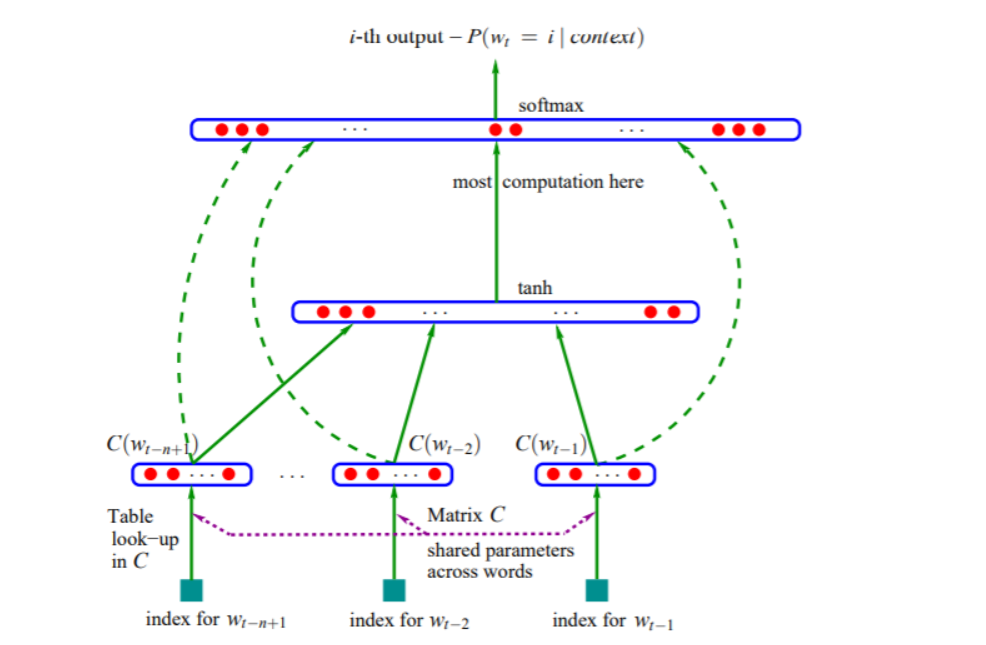
\includegraphics[width=\linewidth]{first_neural_lm}
	\captionof{figure}{Схема первой нейросетевой языковой модели}
	\label{fig:first_neural_lm}
\end{figure}

Следующий прорыв в языковом моделировании случился в 2013 году. Это связано с появлением Word2Vec --- универсальными векторными представлениями слов, разработанными Google. Векторные представления обучены на большом объеме данных, что позволяет хорошо отражать смысл слов. Это значит, что схожим по смыслу и значения словам будут соответствовать близкие по косиноснуму расстоянию вектора. Также исследования показали, что такие представления имеют некоторую линейную зависимость, которая выражается в подобных примерах: $king - man + woman \approx queen$.
Представления Word2Vec могут быть получены на больших объемах неразмеченных текстовых данных с помощью двух методов: Skip-gram и Continous Bag of Words (CBoW). Skip-gram основан на предсказании по данному слову его контекста, а CBoW наоборот --- пытается угадать слово по заданному контексту (Рис. \ref{fig:skipgram_cbow}). Также есть способы улучшить качество векторов и скорость сходимости, например, negative sampling, при котором кроме приближения схожих слов семплируются несколько случайных, и алгоритм пытается «отдалить» друг от друга слова, отличающиеся по смыслу.

\begin{figure}[ht]
	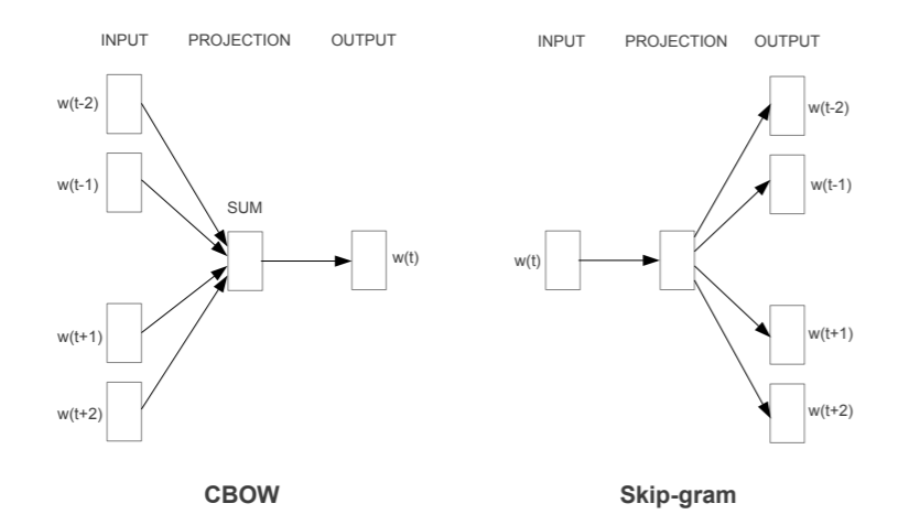
\includegraphics[width=\linewidth]{skip_gram_cbow}
	\captionof{figure}{Skip-gram и CBoW}
	\label{fig:skipgram_cbow}
\end{figure}

Через год после успеха Word2Vec появился GloVe --- аналогичные векторные представления слов, которые показали себя лучше для ряда задач: поиск схожих слов и NER (Рис. ~\ref{fig:glove_vs_word2vec}). GloVe отличается исходными данными для обучения, а также основан на более сложном алгоритме.~\cite{twds-lm-history}

\begin{figure}[ht]
	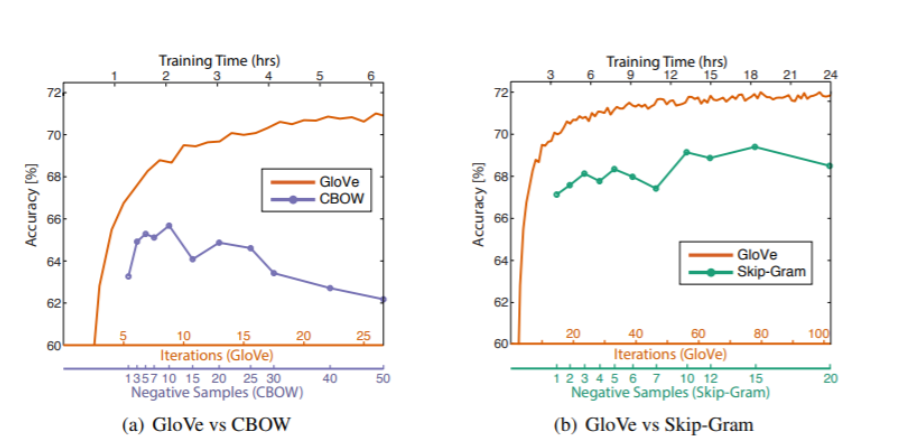
\includegraphics[width=\linewidth]{glove_vs_word2vec}
	\captionof{figure}{GloVe vs Word2Vec}
	\label{fig:glove_vs_word2vec}
\end{figure}

Одновременно с GloVe в 2014 году были созданы сверточные нейронные сети ~\cite{kalchbrenner-etal-2014-convolutional}. Основной сферой применения сверточных сетей является компьютерное зрение, так как по своей природе они наиболее удачно подходят для обработки изображений, однако их можно применять и к текстовым данным. Наряду с рекуррентными сетями, сверточные сети были одним из основных направлений исследований в NLP.

Несмотря на то, что рекуррентные сети являются наиболее очевидным выбором для работы с последовательностями переменной длины, их обучение затруднялось особенностями архитектуры, а также такими феноменами, как затухающие и взрывающиеся градиенты, которые влиялии на вычислительную стабильность обратного распространения градиентов. Довольно большой вклад в решение данных проблем внес phd тезис~\cite{sutskever2013training}, в котором приводились результаты успешных экспериментов для различных задач, не только языкового моделирования, которые доказали возможность качественного обучения рекуррентных сетей.

Следующим шагом в развитии моделей для обработки последовательностей были Sequence to Sequence модели (seq2seq). В этой структуре нейронная сеть кодировщика обрабатывает предложение по одному токену и сжимает его в векторное представление; затем нейронная сеть декодера предсказывает выходные символы на основе состояния кодировщика, принимая в качестве входных данных на каждом шаге ранее предсказанный символ (Рис. \ref{fig:seq2seq})

\begin{figure}[ht]
	\centering
	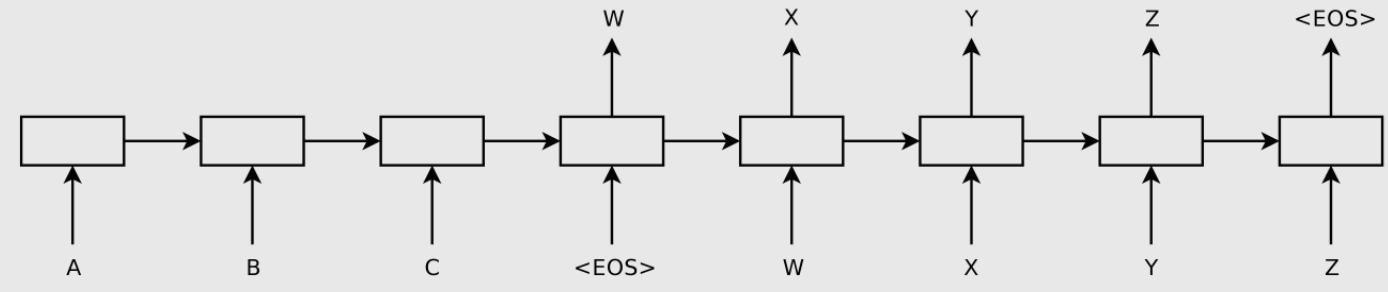
\includegraphics[width=\linewidth]{seq2seq2014}  
	\caption{ Схема seq2seq модели }
	\label{fig:seq2seq}
\end{figure}

Seq2seq благодаря своей гибкости в настоящее время является основным фреймворком для задач генерации естественного языка, при этом различные модели берут на себя роль кодировщика и декодера. Важно отметить, что модель декодера может быть обусловлена не только последовательностью, но и произвольными представлениями. Это позволяет, например, генерировать заголовок на основе изображения (Image Captioning)~\cite{image-captioning}. Здесь в качестве кодировщика применяется сверточная сеть, которая выдает сжатые представления изображений. Далее этот вектор идет на вход декодера, который выдает одно за другим слова заголовка (Рис \ref{fig:image_captioning}).
\begin{figure}[ht]
	\centering
	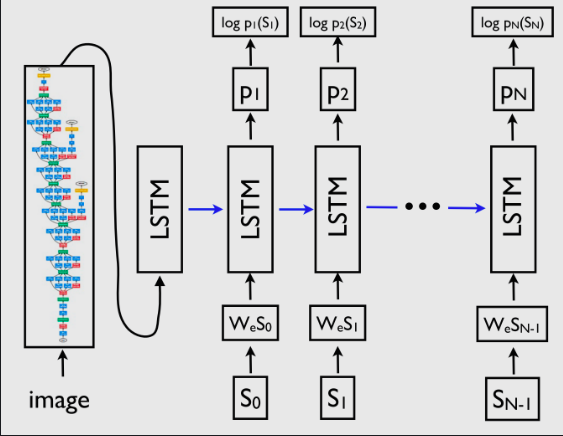
\includegraphics[width=\linewidth]{image_captioning}  
	\caption{ Архитектура seq2seq модели для генерации заголовков к изображениям }
	\label{fig:image_captioning}
\end{figure}

У модели seq2seq есть один значитеьный недостаток, который ограничивает качество моделей, --- вся входная информация сжимается в один вектор, который в дальнейшем используется в рекуррентной сети. Это приводит к тому, что после нескольких применений декодера информация о входном объекте теряется, что ограничивает качество модели. С этим борется механизм внимания, или Attention.

Механизм внимания является одним из основных нововведений в нейронном машинном переводе (NMT) и ключевой идеей, которая позволила моделям NMT превзойти классические системы машинного перевода на основе фраз. Attention позволил решить основную проблему seq2seq моделей, предоставляя декодеру возможность оглянуться назад на скрытые состояния исходной последовательности, которые затем предоставляются в качестве дополнительных входных данных для декодера (Рис. \ref{fig:attention}).

\begin{figure}[ht]
	\centering
	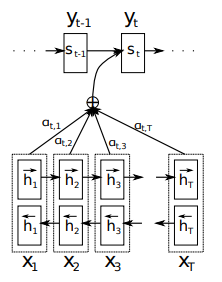
\includegraphics[width=200pt]{attention_layer}  
	\caption{ Механизм attention }
	\label{fig:attention}
\end{figure}

Формула вероятности $P(y_i|y_{<i}, x)$, где $x$ --- это выход кодировщика, для модели attention имеет вид (\ref{eq:attention_1}):
\begin{equation}
	P(y_i|y_1,\dots,y_{i-1}, x) = g(y_{i-1}, s_i, c_i),
	\label{eq:attention_1}
\end{equation} где $s_i$ --- это последнее скрытое состояние рекуррентной сети, а вектор $c_i$ равен взвешенной сумме скрытых состояний рекуррентной сети (\ref{eq:attention_2} -- \ref{eq:attention_4}).

\begin{equation}
	c_i = \sum_{j=1}^{T_x}{\alpha_{ij}h_j}
	\label{eq:attention_2}
\end{equation}

\begin{equation}
	a_{i,j} = \frac{exp(e_{ij})}{\sum_{k=1}^{T_x}{e_{ik}}}
	\label{eq:attention_3}
\end{equation}

\begin{equation}
	e_{ij} = a(s_{i-1}h_j)
	\label{eq:attention_4}
\end{equation}

Матрица $e$ служит для соответствия входа и выхода модели, оценивая, насколько хоошо соотносятся $i$-ый символ входной и $j$-ый символ выходной последовательностей.~\cite{attention}

Следующим прорывом в области NLP стало появление архитектуры трансформеров (рис. \ref{fig:transformer}) и переход к pre-trained моделям. На данный момент все state of the art модели в NLP так или иначе используют трансформеры. Их появление позволило создавать модели, состоящие из миллиардов параметров, обученные на сотнях GPU с использованием многих терабайтов данных. К наиболее популярным предобученным трансформерам относятся BERT, ALBERT, ROBERTA, ELMO, ERNIE, XLNET, GTP-2, T5 и другие.

\begin{figure}[ht]
	\centering
	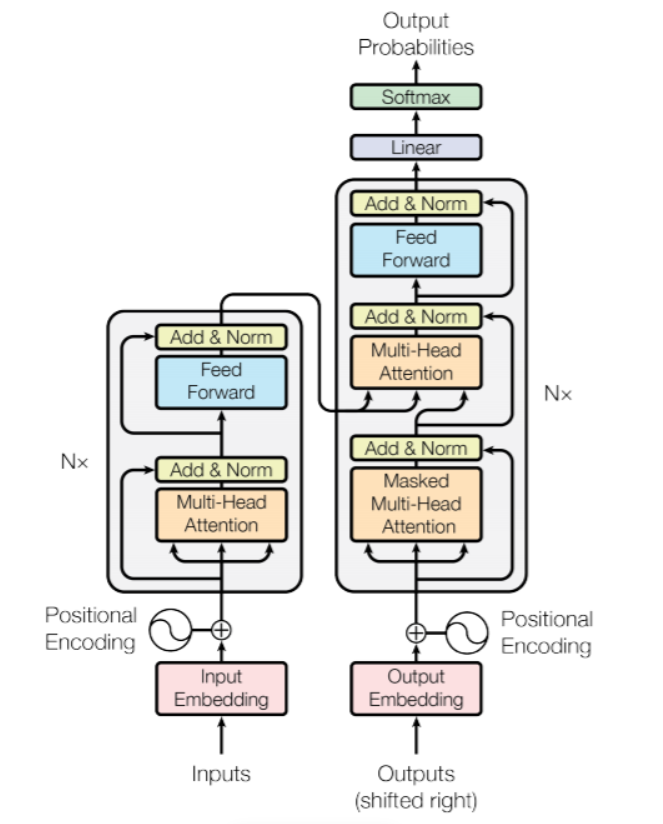
\includegraphics{transformer}  
	\caption{ Структура блока трансформера}
	\label{fig:transformer}
\end{figure}

\subsection{N-грамные модели}
\label{sub:domain:n_gram}

Как уже было показано ранее, мы можем оценивать вероятности конкретных последовательностей по формуле (\ref{eq:conditional_proba}). Основная задача заключается в получении вероятностей $P(y_i|y_{<i})$. Наиболее очевидный способ --- узнать, какая часть последовательностей $y_1, y_2,\dots, y_{t-1}$ предшествует $y_t$ (\ref{eq:ngram}).
\begin{equation}
	P(y_t|y_1,y_2,\dots,y_{t-1}) = \frac{N(y_1,y_2,\dots,y_t)}{N(y_1,y_2,\dots,y_{t-1})},
	\label{eq:ngram}
\end{equation} где $N(y_1,\dots,y_k)$ -- количество раз, которое последовательность $y_1,\dots,y_k$ встречается в тексте. У данного способа довольно много недостатков: пересчитывать для последовательностей длиннее нескольких символов дорого, и значительная часть более длинных последовательностей в тексте не встречается, что даст нам нулевую вероятность. Чтобы этого избежать, сделаем предположение о Том, что текущее состояние зависит от контекста фиксированной длины. Формально это выражается в виде (1.7).
\begin{equation}
	P(y_t|y_1,y_2,\dots,y_{t-1}) = P(y_t|y_{t-n+1}, y_{t-n+2},\dots,y_{t-1})
\end{equation}
Для конкретных значений получим
\begin{itemize}
	\item[при] $n = 3$ (trigram): $P(y_t|y_1,y_2,\dots,y_{t-1}) = P(y_t|, y_{t-2},y_{t-1})$
	\item[при] $n = 2$ (bigram): $P(y_t|y_1,y_2,\dots,y_{t-1}) = P(y_t|, y_{t-1})$
	\item[при] $n = 1$ (unigram): $P(y_t|y_1,y_2,\dots,y_{t-1}) = P(y_t)$
\end{itemize}

Далее можно столкнуться с проблемой, что либо числитель, либо знаменатель в формуле вероятности будет равен нулю. Для борьбы с нулем в знаменателе можно использовать:

\begin{itemize}
	\item Backoff, при котором мы просто уменьшаем контекст. То есть если $P(y_t|y_{t-n+1},\dots,y_{t-1}) = 0$, можно попробовать посчитать $P(y_t|y_{t-n+2},\dots,y_{t-1})$
	\item Linear interpolation. Это более качественный подход, в котором вероятность формируется сразу из нескольких n-gram. Например, для уни-, би- и триграм получим формулу $P(y_t|y_{t-2}, y_{t-1}) = \lambda_2P(y_t|y_{t-2}, y_{t-1}) + \lambda_1P(y_t|y_{t-1}) + \lambda_0P(y_t)$, где $\lambda_0 + \lambda_1 + \lambda_2 = 1$. Коэффициенты для взвешенной суммы можно подбирать кросс-валидацией на тренировочных данных.
\end{itemize}

Для борьбы с нулем в числителе применяется сглаживание. 

\subsubsection{Laplace smoothing}. Самый простой способ выполнить сглаживание --- добавить единицу ко всем счетчикам n-грамм, прежде чем
мы нормализуем их в вероятности. Этот алгоритм называется
Laplace smoothing. Laplace smoothing работает недостаточно хорошо, чтобы его можно было использовать в современных n-граммных моделях, но вводит многие концепции, которые успешно применяются в других статистических моделях, дает неплохой бейзлайн для дальнейшего языкового моделирования, а также используется на практике для других задач, таких как классификация текстовых документов.

Начнем с применения сглаживания Лапласа к вероятностям униграмм.
Напомним, что несглаженная оценка максимального правдоподобия вероятности униграммы является частным случаем для формулы (1.6) и имеет вид (\ref{eq:unigram_proba}):

\begin{equation}
	\label{eq:unigram_proba}
	P(w_i) = \frac{c_i}{N},
\end{equation}
\begin{explanation}
	где $w_i$ -- оцениваемое слово, $c_i$ -- сколько раз $w_i$ встречалось в тексте, \\$N$ -- общее число токенов.
\end{explanation}

Laplace Smoothing просто добавляет единицу к каждому счетчику (отсюда и его альтернативное название — сглаживание с добавлением единицы). Поскольку в словаре есть V слов, и каждое из них было увеличено, нам также необходимо скорректировать знаменатель, чтобы учесть дополнительное V (\ref{eq:laplace_unigram}).

\begin{equation}
	\label{eq:laplace_unigram}
	P(w_i) = \frac{c_i + 1}{N + V},
\end{equation}

Вместо того, чтобы менять и числитель, и знаменатель, удобно
описать, как алгоритм сглаживания влияет на числитель, определив скорректированное значение счетчика $c_i$ по формуле (\ref{eq:laplace_numerator}):

\begin{equation}
	\label{eq:laplace_numerator}
	c_i^* = (c_i + 1) \cdot \frac{N}{N + V}
\end{equation}

Сглаживание можно также рассматривать как это дисконтирование (понижение) некоторых ненулевых значений счетчиков для того, чтобы перераспределить вероятностную массу и получить ненулевые значения для слов, которые наша модель не знает. ~\cite{n_grams}

\subsubsection{Add-k}. Одной из альтернатив сглаживанию с добавлением единицы является перемещение немного меньшего количества вероятностной массы. Вместо того, чтобы добавлять 1 к каждому значению счетчика, мы добавляем некоторую величину $k$, которая обычно значительно меньше 1. Поэтому данный алгоритм называется Add-k smoothing (\ref{eq:add_k}).

\begin{equation}
	\label{eq:add_k}
	P^*_{Add-k}(w_n|w_{n-1}) = \frac{N(w_{n-1}w_n) + k}{N(w_{n-1}) + kV}
\end{equation}

Для использования Add-k сглаживания необходимо подбирать оптимальное значение k на тренировочных данных, например, при помощи кросс-валидации. несмотря на то, что add-k полезен для некоторых задач (включая классификацию текста), для языкового моделирования он все еще плох из-за больших дисперсий счетчиков и зачастую неуместного дисконтирования.

\subsubsection{Backoff и интерполяция}. Описанное выше дисконтирование позволяет решить проблему проблему n-грамм с нулевой вероятностью. Однако в таком случае мы используем не всю имеющуюся информацию о тренировочных данных, что значительно влияет на качество. Если мы пытаемся посчитать $P(w_n|w_{n-2}w_{n-1})$, но в тексте такая триграмма никогда не встречалась, то мы вместо нее можем использовать вероятность биниграммы $P(w_n|w_{n-1})$. Аналогично если нет данных о биграмме $P(w_n|w_{n-1})$, вместо нее применяем вероятность $P(w_n)$.

Другими словами, полезно использовать меньше контекста для генерализации последовательностей, которые наша модель не выучила. Есть два способа применять данный подход:

\begin{itemize}
	\item Backoff: используется триграмма, если она хоть раз встречалась в тренировочных данных, иначе используем биграмму и т. д. Мы итеративно снижаем контекст, если наша модель не имеет информации о данном контексте.
	\item Интерполяция: вместо одной n-граммы используется линейная комбинация нескольких n-грамм, с подобранными на тренировочных данных весами (\ref{eq:interpolation})
	\begin{equation}
		\hat{P}(w_n|w_{n-2}w_{n-1}) = \lambda_1 P(w_n) + \lambda_2 P(w_n|w_{n-1}) + \lambda_3 P(w_n|w_{n-2}w_{n-1})
		\label{eq:interpolation},
	\end{equation}
	\begin{explanation}
		где $\lambda_i$ -- вес i-ой n-граммы, $\sum_{i}{\lambda_i} = 1$
	\end{explanation}
\end{itemize}

В более сложной версии линейной интерполяции каждый вес $\lambda$ вычисляется в зависимости от контекста. Тогда если для какой-то биграммы у нас будут очень точно оценена ее вероятность, то мы полагаем, что вероятность триграммы будет более достоверная, и мы придаем ей больший вес при интерполяции (\ref{eq:improved_interpolation}).

\begin{equation}
	\begin{split}
	\hat{P}(w_n|w_{n-2}w_{n-1}) = \lambda_1(w_{n-2:n-1}) P(w_n) + \lambda_2(w_{n-2:n-1}) P(w_n|w_{n-1}) + \\ \lambda_3(w_{n-2:n-1}) P(w_n|w_{n-2}w_{n-1})
	\end{split}
	\label{eq:improved_interpolation}
\end{equation}

При таком подходе значения $\lambda$ вычисляются на отложенной выборке. Для этого довольно часто применяется EM алгоритм.

\subsubsection{Katz backoff}. Чтобы backoff модель давала правильное распределение вероятностей, мы вынуждены дисконтировать n-граммы более высокого порядка, чтобы сохранить некоторую вероятностную массу для n-грамм более низкого порядка. Как и в случае сглаживания с добавлением единицы, если n-граммы более высокого порядка не дисконтированные, и мы просто использовали недисконтированную вероятность MLE, то как только мы
заменили n-грамму с нулевой вероятностью n-граммой более низкого порядка, мы бы добавить массу вероятности, а общая вероятность для всех возможных строк будет больше 1. Поэтому, нам понадобится функция $\alpha$, чтобы распределить эту вероятностную массу на меньший порядок n-грамм. ~\cite{n_grams}

Один из видов такого перераспределения вероятностей называется Katz backoff. В данном алгоритме мы полагаемся на сглаженную вероятность P, если мы видели эту n-грамму раньше (т.е. если
у нас есть ненулевые значения). В противном случае мы рекурсивно уменьшаем контекст и смотрим на вероятность (N-1)-граммы. Значения при таком рекурсивеом спуске вычисляются по формуле (\ref{eq:maxim_katz}):

\begin{equation}
	P_{BO}(w_n|w_{n-N+1:n-1}) = 
	\begin{cases}
		P^*(w_n|w_{n-N+1:n-1}), & \mbox{if } C(w_{n-N+1:n}) > 0 \\ \alpha(w_{n-N+1:n-1})P_{BO}(w_n|w_{n-N+2:n-1}), & \mbox{otherwise.}
	\end{cases}
	\label{eq:maxim_katz}
\end{equation}

\subsubsection{Kneser-ney smoothing}. Одним из наиболее часто используемых и наиболее эффективных методов сглаживания n-грамм является алгоритм Kneser-Ney ~\cite{kneser_ney}. Kneser-Ney берет свое начало в методе, называемом абсолютным дисконтированием.

Интуиция, стоящая в основе абсолютного дисконтирования, заключается в том, что, поскольку у нас уже есть хорошие оценки для часто встрачающихся биграмм, небольшая скидка
$d$ на них особо не повлияет. При этом большим изменениям подвергнутся редкие биграммы, вероятностям которых мы и так не можем полностью доверять, и на практике, их снижение положительно сказывается на качестве модели. Уравнение абсолютной интерполяции выглядит следующим образом (\ref{eq:absolute_discounting}):

\begin{equation}
	P_{AD}(w_i|w_{i-1}) = \frac{C(w_{i-1}, w_i) - d}{\sum_v{C(w_{i-1}, v)}} + \lambda(w_{i-1})P(w_i)
	\label{eq:absolute_discounting}
\end{equation}

Дисконтирование Кнезера-Нея ~\cite{kneser_ney} дополняет абсолютное дисконтирование более сложным способом обработки распределения униграмм низшего порядка. Вместо $P(w)$, что отвечает на вопрос «Насколько вероятно $w$?», мы хотели бы создать модель униграммы, которую назовем $P_{continuation}$, которая отвечает на вопрос «Насколько вероятно, что w появится в качестве продолжения?».  Интуиция Кнезера-Нея лежит в основе нашей оценки $P_{continuation}$ от количества различных контекстов, в которых появлялось слово w, то есть от количества биграмм, которые он завершает. Каждая биграмма была каким-то продолжением в новом контексте. Мы предполагаем, что слова, которые появлялись в большем количестве контекстов в
прошлом, скорее всего, также появится в каком-то новом контексте. Количество раз слово w появляется как новое продолжение, может быть выражено в виде (\ref{eq:extension_count}):

\begin{equation}
	P_{continuation}(w) \propto |{v: C(vw) > 0}|
	\label{eq:extension_count}
\end{equation}

Чтобы получить из данной величины вероятность, нормализуем ее по общему количеству известных модели биграмм (\ref{eq:extension_proba}).

\begin{equation}
	P_{continuation} = \frac{|{v:C(vw) > 0}|}{|{(u', w'): C(u', w') > 0}|}
	\label{eq:extension_proba}
\end{equation}

Аналогичным образом оценивается количество слов, которые предшествуют $w$ по формуле (\ref{eq:predicate_proba_or_smth_idk}).

\begin{equation}
	P_{continuation(w)} = \frac{|{v:C(vw) > 0}|}{\sum_{w'}{|{v:C(vw') > 0}|}}
	\label{eq:predicate_proba_or_smth_idk}
\end{equation}

Итоговое уравнение для Interpolated Kneser-Ney smoothing для биграмм принимает вид (\ref{eq:kneser_ney}):

\begin{equation}
	P_{KN}(w_i|w_{i-1}) = \frac{max(C(w_{i-1}w_i) - d, 0)}{C(w_{i-1})} + \lambda(w_{i-1}) P_{continuation}(w_i),
	\label{eq:kneser_ney}
\end{equation}
\begin{explanation}
	где $\lambda$ -- нормализующая константа, рассчитываемая по формуле (\ref{eq:lambda_for_KN}):
\end{explanation}

\begin{equation}
	\lambda(w_{i-1}) = \frac{d}{\sum_v{C(w_{i-1}v)}}|{w:C(w_{i-1}w) > 0}|
	\label{eq:lambda_for_KN},
\end{equation}

Первый член \ref{eq:lambda_for_KN} $\frac{d}{\sum_v{C(w_{i-1}v)}}$ -- коэффициент еормализации дисконтирования, второй член $|{w:C(w_{i-1}w) > 0}|$ -- количество различных слов, которые могут следовать за $w_{i-1}$, или количество раз, которое мы применяем дисконтирование.

Обобщенная формула Kneser-Ney имеет вид (\ref{eq:i_actualy_once_coded_this_shit}):

\begin{equation}
	P_{KN}(w_i|w_{i-n+1:i-1}) = \frac{max(c_{KN}(w_{i-n+1:i})-d, 0)}{\sum_v{c_{KN}(w_{i-n+1:i-1}v)}} + \\ \lambda(w_{i-n+1:i-1})P_{KN}(w_i|w_{i-n+2:i-1})
	\label{eq:i_actualy_once_coded_this_shit}
\end{equation}
\begin{explanation}
	где значение $c_{KN}$ зависит от того, считаем ли старшую n-грамму при \\ интерполяции (\ref{eq:KN_counts}).
\end{explanation}
\begin{equation}
	c_{KN}(\cdot) = \begin{cases} 
		count(\cdot), & \mbox{for the highest order }\\ 
		continuationcount(\cdot) & \mbox{for lower orders}
	\end{cases},
	\label{eq:KN_counts}
\end{equation}
\begin{explanation}
	где $continuationcount$ описывает количество уникальных однословных \\ контекстов для $\cdot$
\end{explanation}

При завершении рекурсии, униграммы интерполируются равномерным распределением (\ref{eq:KN_termination}):

\begin{equation}
	P_{KN}(w) = \frac{max(c_{KN}(w) - d, 0)}{\sum_{w'}{c_{KN}(w')}} + \lambda(\epsilon)\frac{1}{V},
	\label{eq:KN_termination}
\end{equation}
\begin{explanation}
	где $\epsilon$ описывает пустую строку.
\end{explanation}

Если мы хотим учитывать незнакомые слова $\text{<UNK>}$, то оно включается как обычный элемент словаря с количеством 0, и его вероятность будет по формуле (\ref{eq:KN_termination}) равна $\frac{\lambda{\epsilon}}{V}$.

Наилучшая версия алгоритма Kneser-Ney называется modified Kneser-Ney smoothing и описана в статье ~\cite{modified-kneser-ney}. Вместо использования одного значения $d$, в ней предлагается использовать три различных коэффициента дисконтирования $d_1$, $d_2$ и $d_{3+}$, что позволило превзойти начальную версию алгоритма. ~\cite{n_grams}

\subsection{Нейросетевые модели}
\label{sub:domain:neural}

Аналогично n-граммным моделям, нейросетевые языковые модели учатся предсказывать вероятность $P(y_1, y_2, \dots, y_n)$ последовательности \\ $(y_1, y_2, \dots, y_n)$, которая раскладывается в произведение условных вероятностей по формуле $\ref{eq:conditional_proba}$.

Входными данными нейросетевой модели являются токены \\ $(y_1, y_2, \dots, y_{n-1})$. Результатом, который мы хотим получить, является распределение вероятностей по различным значениям, которые может принимать $y_n$, представляющее собой вектор фиксированной длины. Стоит отметить, что размерность этого вектора зависит от размера словаря и может быть очень высокой --- до сотен тысяч и даже миллионов с учетом всевозможных слов. Входные данные, в свою очередь, не имеют фиксированной длины, и чем больше токенов приходит на вход, тем более сложной и вычислительно затратной становится задача языкового моделирования.

На данный момент существуют три основных вида нейросетей, применяемых для языкового моделирования: сверточные, рекуррентные и трансформеры. ~\cite{neural_lms}

\subsubsection{Рекуррентные сети}. Рекуррентные нейронные сети (RNN) привлекательны для языкового моделирования, потому что у них фиксированной длины последовательности. То есть, в теории такая сеть способна учитывать контексты любой длины. Тем не менее, это не так просто и не каждая рекуррентная модель с этим справляется. Для начала опишем базовую RNN, которой сложно запоминать длинные зависимости.

По своей структуре базовая RNN мало чем отличается от полносвязной нейронной сети. На вход она получает вектор $x$, и на выходе дает вектор $y$. Отличия заключаются в том, что RNN может обрабатывать последовательность векторов $(x_1, x_2, \dots, x_n)$, выдавая для каждого $x_i$ вектор $y_i$. На выход $y_i$ в момент времени $i$ влияет не только $x_i$, но и вся последовательность $x_1, \dots, x_{i-1}$ входов, полученных до этого момента. Именно это и делает RNN хорошим выбором для работы с последовательностями переменной длины, но также значительно усложняет обучение. Каким-то образом нейросеть должна сохранять историю $(x_i, \dots, x_{i-1})$ в состояние, которое мы назовем $h_{i-1}$, на основе которого можно качественно предсказать $y_{i-1}$. Когда на вход поступает $x_i$, происходит обновление состояния $h_i$. По сути, вектор $x_i$ становится частью истории входных данных, которые видела модель. Затем из $h_i$ создается выходной вектор $y_i$. Формально это можно записать в виде формулы (\ref{eq:recurrent_net}).
\begin{equation}
	\begin{split}
		&h_t = f(h_{t-1}, x_t) \\
		&y_t = g(h_t)
	\end{split}
	\label{eq:recurrent_net}
\end{equation}
\begin{explanation}
	где $f$ --- функции для обновления состояния, \\
	$g$ --- функция для предсказания следующего токена.
\end{explanation}

Данные функции в большинстве случаев представляют собой один линейный слой с последующей функцией активации (\ref{eq:basic_rnn_layer}):
\begin{equation}
	\begin{split}
		&f(h, x) = S_1(W_h \times h + W_x \times x) \\
		&g(h) = S_2(W_y \times h)
	\end{split}
	\label{eq:basic_rnn_layer}
\end{equation}
\begin{explanation}
	где $W_h$, $W_x$, $W_y$ --- веса линейного слоя модели, \\
	где $S_1$, $S_2$ --- функции активации, в случае сигмоиды имеет вид (\ref{eq:sigmoid})
\end{explanation}
\begin{equation}
	\sigma(x) = \frac{1}{1 + e^{-x}}
	\label{eq:sigmoid}
\end{equation}

В случае применения рекуррентной сети для языкового моделирования, последовательность слов $w_1, w_2, \cdots, w_n$ может быть превращена в обучающий пример для этой языковой модели. Для этого мы отдаем по одному токену в сеть, получаем вероятности следующего и максимизируем вероятность следующего токена последовательности. Формально это выглядет следующим образом: пусть модель уже обработала $k$ слов и было получено состояние сети $h_k$. На основе данного состояния можно получить распределение на следующий токен. Получив распределение, мы оптимизируем веса модели таким образом, чтобы максимизировать вероятность токена $w_{k+1}$, так как именно оно встретилось при заданном контексте в нашей последовательности. Для оптимизации чаще всего используется градиентный спуск и кроссэнтропия в качестве функции потерь (\ref{eq:cross_entropy}).
\begin{equation}
	\mathnormal{L} = -\sum{(y\log{p} + (1 - y)\log{(1-p)})}
	\label{eq:cross_entropy}
\end{equation}
\begin{explanation}
	где $y$ --- целевые вероятности, \\
	$p$ --- предсказанные вероятности.
\end{explanation}

Обучаемые параметры — это матрицы весов $W_h$, $W_x$ и $W_y$. $W_h$ описывает влияние текущего вектора состояния $h_i$ на $h_{i+1}$, $W_x$ --- связь $x_{i+1}$ и $h_{i+1}$, а $W_y$ --- влияние $x_{i+1}$ на $y_{i+1}$.

При обучении RNN возникает ряд серьезных проблем. При росте длины контекста градиент должен проходить через все большее число слоев, что приводит к затухающим (крайне близким к 0 либо равным 0) или взрывающимся
(экспоненциально возрастающим, стремящимся к бесконечности) градиентам. Это связано с тем, что происходит фактически возведение в степень матрицы весов при многократном последовательном ее применении к вектору состояния, что ведет к вычислительной нестабильности сети и ее неспособности выучивать более длинные контексты. В связи с этим классическая RNN не находит применения на практике. Вместо нее используют GRU (Gated Recurrent Unit) либо LSTM (Long-Short Term Memory).

GRU во многом работает так же, как базовая RNN. Вход представляет собой последовательность векторов, подающихся в сеть один за другим. GRU поддерживает вектор состояния, фиксируя некоторые ключевые аспекты того, что модель видела раньше. Это состояние в сочетании со следующим входом определяет следующее состояние. ~\cite{neural_lms}

В базовой RNN скрытое состояние изменяется по формуле ($\ref{eq:basic_rnn_layer}$). GRU строит $h_t$ из $h_{t-1}$ и $x_t$ другим образом. Вводится понятие нового состояния $h_{new}(t)$, производного от $h_{t-1}$ и $x_t$. В формулу добавляется фильтр, который позволяет выборочно извлекать информацию из предыдущего состояния. Этот фильтр $s_t$ принимает значение от 0 до 1. Фильтрация представляет собой поэлементное  умножение $h_{i-1}$ на $s_t$. Полное уравнение принимает вид (\ref{eq:gru_gate}):
\begin{equation}
	h_{new}(t) = \tanh{(W_xx_t + W_h(s_t \circ h_{t-1}) + b)}
	\label{eq:gru_gate}
\end{equation}
\begin{explanation}
	где $\tanh$ --- функция активации, вычисляется по формуле (\ref{eq:tanh}), \\
	$b$ --- bias из формулы для линейного слоя $W \times x + b$.
\end{explanation}
\begin{equation}
	\tanh{(\alpha)} = \frac{e^{2\alpha} - 1}{e^{2\alpha} + 1}
	\label{eq:tanh}
\end{equation}

Фильтр $s_t$ задается формулой (\ref{eq:gru_filter_gate}):
\begin{equation}
	s_i = \sigma(Dx_t + Eh_{t-1} + F),
	\label{eq:gru_filter_gate}
\end{equation}
\begin{explanation}
	где $D$, $E$ и $F$ --- обучаемые параметры нейросети.
\end{explanation}

Для изменения скрытого состояния вводится еще один фильтр, $u_t$, который вычисляется по формуле (\ref{eq:gru_update_gate}):
\begin{equation}
	u_t = \sigma(Ax_t + Bh_{t-1} + C),
	\label{eq:gru_update_gate}
\end{equation}
\begin{explanation}
	где $A$, $B$ и $C$ --- обучаемые параметры сети.
\end{explanation}

Изменение скрытого состояния $h_t$ происходит по формуле (\ref{eq:gru_hidden}):
\begin{equation}
	h_t = (1 - u_t) \circ h_{t-1} + u_t \circ h_new(t)
	\label{eq:gru_hidden}
\end{equation}

Использование фильтров, контролирующих, какая информация будет проходить дальше по сети при обработке новых элементов последовательности, позволяет решить ряд проблем классической RNN. GRU обучается намного лучше, решает проблему взрывающихся градиентов и меньше страдает от затухания градиентов, а также позволяет лучше запоминать более длинные контексты. До появления трансформеров, GRU широко применялся для решения различных задач, связанных с обработкой текстовых данных, и давал очень неплохое качество. Для языкового моделирования все же чаще применялась модель LSTM, которая имеет небольшое преимущество на длинных последовательностях.

LSTM долгое время была state-of-the-art (SOTA) моделью языкового моделирования. Ее принцип работы очень схож с GRU, но структура фильтров немного отличается (Рис. \ref{fig:lstm}).

\begin{figure}[ht]
	\centering
	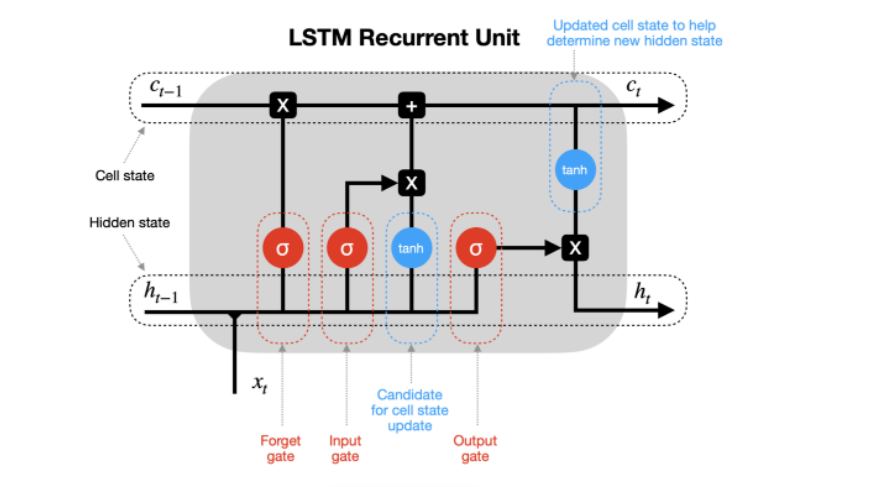
\includegraphics[width=\linewidth]{lstm}  
	\caption{ Структура lstm }
	\label{fig:lstm}
\end{figure}


\subsubsection{Сверточные сети}.  

\subsubsection{Self-attention и трансформеры}

\subsection{Современные подходы к языковому моделированию}
\label{sub:domain:curr}

\subsection{Метрики для языковых моделей}




\lstset{style=fsharpstyle}

\section{Используемые технологии} 
\label{sec:practice:technology_used}

\subsection{Язык Python}

Python — высокоуровневый язык программирования общего назначения с динамической строгой типизацией и автоматическим управлением памятью, ориентированный на повышение производительности разработчика, читаемости кода и его качества, а также на обеспечение переносимости написанных на нём программ. Язык является полностью объектно-ориентированным — всё является объектами. Синтаксис ядра языка минималистичен, за счёт чего на практике редко возникает необходимость обращаться к документации. Сам же язык известен как интерпретируемый и используется в том числе для написания скриптов. Недостатками языка являются зачастую более низкая скорость работы и более высокое потребление памяти написанных на нём программ по сравнению с аналогичным кодом, написанным на компилируемых языках. 
Python стал главным языком мира машинного обучения за счет того, что:

\begin{itemize}
	\item Python обладает большим выбором библиотек и фреймворков.  В научных расчетах используется Numpy, в продвинутых вычислениях — SciPy, в извлечении и анализе данных при помощи методов классического машинного обучения — SciKit-Learn. Для нейросетевых моделей используются такие фреймворки как Tensorflow (больше распространен в production сфере в силу возможностей для реализации распределенных вычислений на нескольких машинах) и Pytorch (распространен в академической среде в силу своей простоты). При этом Python является языком общего назначения, поэтому кроме инструментов для сложных вычислений обладает всеми типичными для других языков инструментами (к примеру, микро-фреймворк для создания веб-сервисов Flask), которые также используются для построения полноценных приложений на основе машинного обучения
	\item Понятность. Python предоставляет разработчику уровень абстракций и конструкций обеспечивающих понятность написанных программ. Это подходит для машинного обучения, потому что сами алгоритмы машинного обучения сложны для понимания. При работе с Python разработчику не нужно уделять много внимания непосредственно написанию кода: все внимание он может сосредоточить на решении более сложных задач, связанных с машинным обучением. Простой синтаксис языка Python помогает разработчику тестировать сложные алгоритмы с минимальной тратой времени на их реализацию.
	\item Общирная поддержка. Еще одно преимущество Python — это обширная поддержка и качественная документация. Существует множество полезных ресурсов о Python, на которых программист может получить помощь и консультацию, находясь на любом этапе разработки.
	\item Следующее преимущество Python в машинном обучении состоит в его гибкости: например, у разработчика есть выбор между объектно-ориентированным подходом и скриптами. Python помогает объединять различные типы данных. Более того, Python особенно удобен для тех разработчиков, которые большую часть кода пишут с помощью IDE
\end{itemize}
Перечисленные выше факторы объясняют, почему Python так активно используется в сфере машинного обучения. Его простота помогает быстро прототипировать сложные нейросетевые модели, проверять и оценивать различные эксперименты с данными.

\subsection{Jupyter}
\subsection{Pandas}
\subsection{Matplotlib}
\subsection{Sentencepiece}
\subsection{Pytorch}
\subsection{ONNX}


%\section{Архитектура и модули системы} % (fold)
\label{sec:arch_and_mod}

Разработанное программное обеспечение представляет из себя библиотеку кода написанную на языках \fsharp{} и \csharp{}.
Библиотека предназначена для представления модификации классических байесовых сетей, упомянутой на странице~\pageref{page:domain:bayes_mod} в подразделе~\ref{sub:domain:bayes_net}.

\subsection{Типы для работы с графами}
\label{sub:arch_and_mod:graphlib}

Так как в дипломном проекте рассматривается одна из разновидностей графовых моделей, то, очевидно, для представления таких моделей в разрабатываемой библиотеке должна быть часть, отвечающая за представление и работу с графами.
При реализации здесь было несколько альтернативных путей: использовать одну из доступных библиотек для платформы \dotnet{} для работы с графами или реализовать собственную.
Среди готовых библиотек можно было бы использовать QuickGraph\footnote{\url{http://quickgraph.codeplex.com/}}, Directed Graph for .NET\footnote{\url{http://directedgraph4net.codeplex.com/}} или GrapheNET\footnote{\url{http://graphenet.codeplex.com/}}.
Но было принято решение остановиться на варианте, подразумевающем разработку собственных типов для работы с графами.
Это решение было обосновано тем, что вышеуказанные библиотеки являются сложными и содержат в себе очень много функциональности не нужной для решения поставленных задач, в дополнение не было приобретено лишних мегабайтовых внешних зависимостей для библиотеки.

Одним из важных решений, которое было принято в начале проектирования модуля работы с графами, было использование по возможности неизменяемых структур данных.
Это решение выгодно отличает разработанную реализацию от существующих библиотек, от использования которых было принято решение отказаться. 
Существующие библиотеки ориентированы на работу в императивном стиле и с изменяемым состоянием.
Также использование неизменяемых структур данных для реализации типов для представления графов в дальнейшем положительно сказалось на простоте реализации поиска структуры вероятностной сети в алгоритмах вывода структуры по данным.
Часть разрабатываемой библиотеки, содержащая типы для работы с графами, реализована на языке программирования \fsharp{}.
Краткое описание основных особенностей данного языка приведено в подразделе~\ref{sub:practice:fsharp_overview}.
Решение использовать данный язык было продиктовано желанием сократить количество возможных ошибок и размер кодовой базы, необходимой для реализации поставленной задачи, а так же желанием применить в <<боевых>> условиях язык программирования с хорошей поддержкой функционального программирования.

Внутренним представлением графа является неизменяемый словарь, содержащий вложенный неизменяемый мульти"=словарь\footnote{Словарь позволяющий хранить множество значений с одинаковым ключом.}.
Основные определения структуры данных графа приведены в листинге~\ref{lst:arch_and_mod:graph_definition}:
\begin{lstlisting}[style=fsharpstyle,caption={Определение структуры данных для представления графа}, label=lst:arch_and_mod:graph_definition]
/// Graph arc 
type Arc<'T> =
    | Outgoing of 'T
    | Incoming of 'T

/// Immutable Graph class
[<ReferenceEquality; NoComparison>]
type Graph<'Vertex, 'Arc when 'Vertex : comparison and 'Vertex : equality and 'Vertex :> IComparable> = 
    private Graph of Map<'Vertex, MultiMap<'Vertex, Arc<'Arc>>>
\end{lstlisting}

Данная структура данных для представления графа подходит для работы как с неориентированными так и с ориентированными мультиграфами.
Воспринимать граф как ориентированный или нет задача конкретного алгоритма, работающего с графом.
Разработанная библиотека для представления графа предоставляет необходимые операции для манипулирования структурой графа. 
Библиотека также предоставляет небольшое количество алгоритмов для работы с графами, необходимых в рамках решения задач, возникающих при поиске структуры вероятностной сети.
В частности реализованы алгоритмы топологической сортировки, поиска в глубину и ширину, поиска сильно"=связанных компонетов и проверки графа на наличие направленных циклов. 

Одной из особенностей разработанной библиотеки является ориентированность на использование как из языка \fsharp{} в <<функциональном стиле>>, так и из языка \csharp{} "--- в <<императивном>>.
Для реализации данной возможности были учтены рекомендации приведенные в~\cite{fsdg_2010}.
Функциональность разработанной библиотеки покрыта большим набором модульных тестов, написанных с использованием библиотек xUnit\footnote{\url{http://xunit.codeplex.com/}} и Unquote\footnote{\url{http://code.google.com/p/unquote/}}.


\subsection{Представление вероятностной сети}
\label{sub:arch_and_mod:probab_net}

Другой важной частью разработанной библиотеки являются типы для представления и работы с самими вероятностными сетями.
Первостепенными требованиями, поставленными перед началом проектирования типов, были следующие пункты:
\begin{itemize}
  \item Типы предназначены для представления модификации классических байесовых сетей, упомянутой в разделе~\ref{sub:domain:bayes_net} на странице~\pageref{page:domain:bayes_mod}.
  \item Представление сети должно быть <<многослойным>>.
  Под <<многослойностью>> понимается возможность расширения представления сети дополнительными <<слоями>> атрибутов, с целью увеличения количества сценариев, в которых данные типы пригодны к использованию.
  Например, в случае когда нужно знать лишь структуру сети можно использовать лишь информацию о структуре "--- граф.
  Для проведения статистического вывода суждений добавляется дополнительный <<слой>>, содержащий талицы условных и безусловных вероятностей.
  В случаях, когда нужно отображать сеть пользователю, добавляется еще один <<слой>>, содержащий дополнительную информацию о переменных и их состояниях. 
  \item Сеть должна предоставлять возможность отмены вносимых в нее изменений, т.\,е. по сути поддерживать версионность.
  \item Сеть должна предоставлять возможность валидации её структуры. 
\end{itemize}

Приняв во внимание приведенные выше требования были приняты следующие решения:
\begin{itemize}
  \item Необходимо разработать отдельные типы для представления вершин вероятностной модели и связей между переменными в этой модели.
  В разработанной библиотеке за это отвечают типы \lstinline!Node<'T>! и \lstinline!Link<'T>!, содержащие информацию о переменных, таблицы распределения и дополнительные атрибуты.
  Использование параметрического полиморфизма в реализации данных типов играет ключевую роль в обеспечении <<многослойности>> и расширяемости представления вероятностной сети.
  \item Необходимы типы для представления распределения.
  В предложенной реализации был разработан тип для представления безусловного распределения случайной величины, эта таблица хранится в сети как один из аттрибутов типа \lstinline!Node<'T>!, и тип для представления условного распределения пары случайных величин, экземпляр данного типа хранится как аттрибут связи между переменными "--- \lstinline!Link<'T>!.
  Было сочтено целесообразным в качестве внутренней реализации таблиц распределения использовать готовую библиотеку для работы с матрицами и другими математическими объектами и понятиями "--- Math.NET Numerics\footnote{\url{http://numerics.mathdotnet.com/}}.
  Соответственно в предложенной реализации использовались типы \lstinline!Vector<float>! и \lstinline!Matrix<float>! и сопутствующие операции над ними.
  Использование данной библиотеки позволило сократить объём сопутствующего кода, необходимого для реализации библиотеки для работы с вероятностными сетями, также уменьшив множество потенциальных ошибок реализации.
  В данном случае преимущества от использования библиотеки превысили затраты на добавление и поддержку дополнительных зависимостей.

  \item Требование возможности отмены изменений вносимых в вероятностную сеть привело к реализации сети, как и в случае типов для представления графов, к реализации сети как неизменяемой структуры данных.
  Все операции, при условии использования специальных функций, возвращают новый экземпляр сети, оставляя старый не изменённым.
  Подобная реализация типов автоматически дает возможность производить версионирование экземпляров типа, т.\,к. всегда есть доступ к изменённой копии и исходному экземпляру.
  С первого взгляда данный подход кажется очень расточительным по памяти, но на самом деле оказывается, что все с точностью до наоборот, т.\,к. обычно, и в данном конкретном случае, при модификации неизменяемой структуры данных большая часть структуры разделяется между копией и исходной структурой, а физически копирование памяти происходит лишь в тех местах, которые действительно необходимо было поменять.
  Для убедительности, сказанное проиллюстрировано на рисунке~\ref{fig:arch_and_mod:probab_net:immutable_ds_modification}.

  \item Валидация сети происходит на этапе её построения и модификации.
  Дополнительно существуют функции для проверки структуры сети на ацикличность.
  Ацикличность ориентированного графа проверяется с помощью алгоритма нахождения компонент сильной связности Косарайю\footnote{\url{http://en.wikipedia.org/wiki/Kosaraju's_algorithm}}.

\end{itemize}

\begin{figure}[ht]
\centering
  \begin{subfigure}[b]{0.41\linewidth} 
    \centering
    \includegraphics[scale=0.63]{persistent_tree.pdf}  
    \caption{}
  \end{subfigure}
  \begin{subfigure}[b]{0.58\linewidth} 
    \centering
    \includegraphics[scale=0.63]{persistent_tree_mod.pdf}  
    \caption{}
  \end{subfigure}
  \caption{ Пример разделения структуры в неизменяемых структурах данных: 
            а "--- исходное дерево;
            б "--- измененное дерево, добавлена вершина \textit{e};}
  \label{fig:arch_and_mod:probab_net:immutable_ds_modification}
\end{figure}

В результате получилось довольно простое и расширяемое представление сети, основное определение которого приведено в листинге~\ref{lst:arch_and_mod:probab_net:bnet_definition}.
Параметризация типа параметрами \lstinline!'NodeAttributes! и \lstinline!'LinkAttributes! и расширяемое устройство типов \lstinline!Node<'T>! и \lstinline!Link<'T>! позволяет достигнуть заявленной расширяемости представления сети и её <<многослойности>>.
Библиотека содержит предопредёленные типы, для представления уровней.
Параметризация типа \lstinline!BNet<unit, unit>! представляет структуру сети и таблицы распределения.
<<Слой>> с дополнительными аттрибутами, планируемыми для использования в алгоритмах статистического вывода суждений представлен типами \lstinline!NodeAttributes<'Annotations>! и \lstinline!LinkAttributes!, но на момент защиты дипломного проекта, из-за неготовой реализации алгоритмов статистического вывода суждений, данные типы содержат не все необходимые атрибуты для работы таких алгоритмов, а лишь прогнозируемых заготовки.
Дополнительный <<слой>>, потенциально необходимый при построении пользовательских приложений, представлен типом \lstinline!VarAnnotations!.
Данный тип содержит дополнительную информацию о переменной, такую как её название и аннотации возможных значений переменной.
Таким образом, наиболее полное представление сети, содержащее все <<слои>>, в коде параметризуется следующим образом \lstinline!BNet<NodeAttributes<VarAnnotations>, LinkAttributes>!.

\begin{lstlisting}[style=fsharpstyle,caption={Определение структуры данных для вероятностной сети}, label=lst:arch_and_mod:probab_net:bnet_definition]
/// Represents immutable BN. Nodes and links between nodes.
type BNet<'NodeAttributes, 'LinkAttributes> = 
    private { nodes: Map<int, Node<'NodeAttributes>>;
              links: Map<int * int, Link<'LinkAttributes>>;
              graph: Graph<int, unit>; } 
\end{lstlisting}

Таким образом, использование параметрического полиморфизма и не\-изменяемых типов данных, позволило добиться поставленных при проектировании целей, а также довольно легкой возможности расширять сеть в дальнейшем.

\subsection{Сохранение сети} % (fold)
\label{sub:arch_and_mod:net_persistence}

Помимо функциональности, связанной с представлением, манипуляцией и выведением структуры сети, разработанная библиотека предоставляет возможность импорта и экспорта вероятностной сети из и в различные форматы.
Т.\,к. библиотека предназначена для работы с модификацией вероятностных сетей, отличающейся в нескольких ключевых моментах от классических байесовых сетей, то нельзя было использовать общепринятые форматы для хранения сетей во внешней памяти и необходимо было разработать свой формат.
Разработанный формат хранения сетей основывается на XML и предназначен для полного сохранения состояния представления сети, используемого в программе.
Данный формат в большей степени похож на ручную сериализацию, чем на удобный формат для обмена вероятностными сетями.
Пример сети, представленной в данном формате, приведен в листинге~\ref{lst:arch_and_mod:net_persistence:bnxml}.

У разработанного формата есть существенный недостаток, его <<понимает>> только разработанная библиотека.
В связи с тем, что в данном дипломном проекте основной целью является реализация лишь малой части возможных операций над вероятностными сетями "--- построение структуры по данным, целесообразно было добавить в библиотеку, хотя и весьма ограниченную, возможность загрузки и сохранения вероятностных сетей из и в существующие распространённые форматы.
Список поддерживаемых форматов приведён в таблице~\ref{table:arch_and_mod:net_persistence:supported_formats}.
Поддержка нескольких форматов понадобилась потому, что многие существующие программы, которые использовались в различной степени для оценки результатов проделанной работы, поддерживают весьма ограниченный набор форматов.
Таким образом, имея возможность экспортировать сеть, построенную одним из алгоритмов реализованных в разработанной библиотеке по данным, в общеиспользуемый формат можно использовать обученную сеть для статистического вывода суждений и других операций в существующих программах, т.\,к. в данный момент в разработанной библиотеке данная функциональность не реализована.
Отдельно стоит отметить возможность сохранения структуры сети в формат представления графов программы GraphViz\footnote{\url{http://www.graphviz.org/}}.
Данное ПО использовалось с целью визуализации выведенных структур и экспорта полученной визуализации в один из векторных графических форматов.
Утилита dot из состава GraphViz умеет автоматически визуализировать сложные графы наилучшим для отображения образом.

\clearpage
\begin{lstlisting}[language=XML,caption={Пример представления простой вероятностной сети в собственном XML"=формате}, label=lst:arch_and_mod:net_persistence:bnxml]
<network>
  <variables>
    <variable id="1" dim="2" />
    <variable id="2" dim="3" />
  </variables>
  <node_attributes>
    <node variable_id="1"> <answered>false</answered> </node>
    <node variable_id="2"> <answered>true</answered>  </node>
  </node_attributes> 
  <link_attributes>
    <link parent_id="1" child_id="2" />
  </link_attributes>
  <variable_annotations>
    <variable_annotation variable_id="1">
      <name>My variable</name>
      <annotations>
        <label>Yes</label> <label>No</label>
      </annotations>
    </variable_annotation>
    <variable_annotation variable_id="2">
      <name>Color</name>
      <annotations>
        <label>Red</label> <label>Green</label> <label>Blue</label>
      </annotations>
    </variable_annotation>
  </variable_annotations>
  <probability_tables>
    <probability_table variable_id="1">
      <vector>0.2 0.8</vector>
    </probability_table>
    <probability_table variable_id="2">
      <vector>0.4 0.3 0.3</vector>
    </probability_table>
  </probability_tables>
  <forward_probability_tables>
    <forward_probability_table variable_id="2" condition_variable_id="1">
      <matrix nrows="3" ncols="2">0.1 0.2 0.7 0.6 0.1 0.3</matrix>
    </forward_probability_table>
  </forward_probability_tables>
</network>
\end{lstlisting}

\begin{table}[ht]
\caption{Поддерживаемые форматы хранения вероятностных сетей}
\label{table:arch_and_mod:net_persistence:supported_formats}
\centering
  \begin{tabular}{| >{\raggedright}m{0.35\textwidth} 
                  | >{\centering}m{0.27\textwidth} 
                  | >{\centering\arraybackslash}m{0.27\textwidth}|}
  \hline Формат & Поддержка импорта & Поддержка экспорта \\
  \hline Собственный xml"=формат & полная & полная \\
  \hline XMLBIF & частичная & частичная \\
  \hline GeNIe & частичная & отсутствует \\
  \hline GraphViz dot & отсутствует & полная \\
  \hline
  \end{tabular}
\end{table}



\subsection{Представление экспериментальных данных}
\label{sub:arch_and_mod:dataframe}

Немаловажной задачей в обучении и построении структуры сети по данным является представление набора экспериментальных данных в оперативной и постоянной памяти.
В машинном обучении и других областях, связанных с обработкой массивов данных, для хранения данных на диске в большинстве случаев применяется простой текстовый формат \emph{csv} "--- значения, разделённые специальным символом и записанные в текстовый файл построчно.
В разработанной библиотеке также используется данный формат для импортирования экспериментальных данных с диска в память программы для дальнейшей обработки.
Для чтения \emph{csv} файлов используется легковесная внешняя библиотека LumenWorks.Framework.IO\footnote{\url{http://www.codeproject.com/Articles/9258/A-Fast-CSV-Reader}}.

Для представления набора экспериментальны данных в библиотеке присутствует специальный тип "--- DataFrame, который представляет из себя информацию о переменных и, собственно, набор экспериментальных данных в компактном для хранения виде.
Из особенностей реализации стоит упомянуть способ достижения компактности хранения.
При чтении \emph{csv} файла каждому состоянию переменной назначается некоторое 8-битное число, которое является представлением данного состояния в памяти компьютера.
Использование 8"=битного числа с одной стороны ограничивает число возможных состояний одной переменной до \num{256}, с другой стороны "--- данное представление достаточно компактно, чтобы быть пригодным для работы на персональном компьютере разработчика с ограниченным размером ОЗУ и уметь обрабатывать наборы данных из миллионов случаев для десятков переменных.
Одной из дополнительных возможностей DataFrame является возможность производить случайные выборки из имеющегося набора данных.
Данная возможность была использована при реализации алгоритмов вывода структуры вероятностной сети по данным.


\subsection{Байесовы сети Asia и ALARM}
\label{sub:arch_and_mod:asia_and_alarm}

Перед тем как перейти к обсуждению разработанных алгоритмов вывода структуры сети по данным целесообразно обсудить известные сети, которые использовались в качестве моделей для вывода по экспериментальным данным.
Речь пойдет о ставших уже классикой в таких задачах "--- сетях Asia и ALARM.

\subsubsection{Asia }
\label{sub:arch_and_mod:asia_and_alarm:asia}

Байесова сеть Asia является небольшой синтетической сетью, обычно используемой при изучении вероятностных сетей.
Данная вероятностная сеть рассмотрена в работе~\cite{Lauritzen_Spiegelhalter88}.
Искусственная байеосова сеть Asia предназначена для диагностики у пациентов заболеваний связанных с лёгкими.
В перечень диагностируемых болезней входят туберкулёз, рак и бронхит.
Данная сеть имеет восемь бинарных случайных величин.
Структура данной сети приведена на рисунке~\ref{fig:domain:programs:our_impl_plus_asia}~(б) на странице~\pageref{fig:domain:programs:our_impl_plus_asia}.
В таблице~\ref{table:arch_and_mod:asia_and_alarm:asia:vars} приведено описание переменных.

\begin{table}[ht]
\caption{Описание переменных сети Asia}
\label{table:arch_and_mod:asia_and_alarm:asia:vars}
\centering
  \begin{tabular}{| >{\raggedright}m{0.17\textwidth} 
                  | >{\centering}m{0.17\textwidth} 
                  | >{\raggedright\arraybackslash}m{0.57\textwidth}|}
  \hline Переменная & Количество состояний & \begin{center} Примечание \end{center} \\
  \hline VisitAsia & \num{2} & посещал ли пациент Азию \\
  \hline Tuberculosis & \num{2} & болен туберкулёзом \\
  \hline Smoking & \num{2} & курит \\
  \hline Cancer & \num{2} & имеет рак легких \\
  \hline TbOrCa & \num{2} & имеет рак или туберкулёз \\
  \hline XRay & \num{2} & плохая рентгенография \\
  \hline Bronchitis & \num{2} & болен бронхитом \\
  \hline Dyspnea & \num{2} & испытывает удушье \\
  \hline
  \end{tabular}
\end{table}


\subsubsection{ALARM }
\label{sub:arch_and_mod:asia_and_alarm:alarm}

Данная байесова сеть также очень часто рассматривается для оценки качества различных алгоритмов, работающих с вероятностными сетями.
Данная сеть была рассмотрена в работе~\cite{beinlich1989alarm}.
Сеть предназначена для медицинской диагностики, и используется для обработки физиологических наблюдений пациента.
Сеть состоит из переменных трех типов: диагнозов, физиологических показателей и скрытых переменных, которые измерить на практике нельзя.
Данная сеть содержит \num{37} переменных и \num{46} связей между ними.
Максимальное количество переменных"=родителей равно четырём.
Рассматриваемая вероятностная сеть относится к сетям средник размеров.
Данная сеть хорошо изучена и представляет интерес, как модель для оценки качества реализованных в библиотеке алгоритмов.
Структура сети приведена на рисунке~\ref{fig:arch_and_mod:asia_and_alarm:alarm_structure}.
Из-за довольно большого количества переменных здесь не приводится их описание и назначение.
В этой информации нет необходимости для оценки качества реализованных алгоритмов, важно знать общую структуру сети.

\begin{figure}[ht!]
  \hspace{-4ex} % Кривой хак чтобы подвинуть картинку к левому краю страницы
  \includegraphics[scale=0.6]{alarm_reference_net.pdf}  
  \caption{ Структура байесовой сети ALARM }
  \label{fig:arch_and_mod:asia_and_alarm:alarm_structure}
\end{figure}


\subsection{Алгоритм на основе оценки апостериорной вероятности структуры}
\label{sub:arch_and_mod:k2_algorithm}

В данном подразделе рассматривается известный алгоритм, использующий оценку апостериорной вероятности в качестве критерия поиска.
Подробное описание данной оценки и базового алгоритма поиска приведены в работе~\cite{Cooper1991}. 

Формулу~(\ref{eq:domain:k2:model_and_data_prob}) для оценки совместной вероятности на практике напрямую использовать не получится, без введения дополнительных предположений.
Необходимо сделать предположение, что все возможные структуры равновероятны, т.\,е. $P(B_S)$ равно некоторой малой константе $c$.
Таким образом нахождение оптимальной структуры сводится к максимизации формулы~(\ref{eq:arch_and_mod:k2_algorithm:optimization_objective}), т.\,e. задача сводится к нахождению множества вершин"=предков $ \pi_i $ для каждой вершины $X_i$, оптимизирующих целевую функцию~\cite{Cooper1991}.
\begin{align}
  \label{eq:arch_and_mod:k2_algorithm:optimization_objective}
  \max \left[ P(B_S, x^R[n]) \right] = \notag\\
  =
    c \prod_{i = 1}^{R} \max_{\pi_i} 
    \bigg[
      \prod_{j = 1}^{q_i} &% to align formula
      \frac{(\alpha_i - 1)!}
           {(n[\phi_i[j], i, B_S] + \alpha_i - 1)!}
      \prod_{k = 1}^{\alpha_i}
        n[v_{ik}, \phi_i[j], i, B_S]! 
    \bigg] \text{\,.}
\end{align}

Таким образом наивный алгоритм поиска состоит в полном переборе всех возможных родителей для каждой вершины и оптимизации при этом функции~(\ref{eq:arch_and_mod:k2_algorithm:node_optimization_obj}):
\begin{equation}
  \label{eq:arch_and_mod:k2_algorithm:node_optimization_obj}
  g(i, \pi_i) =       
    \prod_{j = 1}^{q_i}
      \frac{(\alpha_i - 1)!}
           {(n[\phi_i[j], i, B_S] + \alpha_i - 1)!}
      \prod_{k = 1}^{\alpha_i}
        n[v_{ik}, \phi_i[j], i, B_S]! \text{\,.}
\end{equation}

На практике наивный вариант не годится из-за большого количества возможных вариантов структур сетей.
В разработанной реализации использовались те же ограничения и стратегия поиска, что и в работе~\cite{Cooper1991}.
Перед началом выполнения алгоритма требуется знание о порядке вершин, таком, что вершины родители всегда находятся раньше вершин потомков.
Схематически алгоритм поиска выглядит следующим образом:

\begin{lstlisting}[mathescape,escapeinside={/*@}{@*/},caption={Псевдокод реализации алгоритма К2}, label=lst:arch_and_mod:k2_algorithm:k2_pseudo]
function k2 =
  (* Input: dataset $x^R[n]$, ordering of variables, u - maximum number of parents per variable.
     Output: for each node, a printout of the parents of the node. *)
  for i in 1 .. R do
    $ \pi_i $ := $ \emptyset $
    $P_{old}$ := $g(i, \pi_i)$; // formula(/*@\ref{eq:arch_and_mod:k2_algorithm:node_optimization_obj}@*/)
    OkToContinue := true;
    while OkToContinue and $|\pi_i| < u$ do
      let z = node in $ \text{Pred}(X_i) - \pi_i $ that maximizes $ g(i, \pi_i \cup {z}) $
      $P_{new}$ := $f(i, \pi_i \cup {z})$
      if $P_{new} > P_{old}$ then
        $P_{old}$ := $P_{new}$;
        $ \pi_i $ := $ \pi_i \cup {z} $
      else OkToContinue := false
    end while
    printfn("Node: ", $X_i$, "Parents of $X_i$:", $\pi_i$)
  end for
end
\end{lstlisting}

В разработанной в рамках дипломного проекта реализации за основу был взят алгоритм К2, приведенный в работе~\cite{Cooper1991}, псевдокод которого показан в листинге~\ref{lst:arch_and_mod:k2_algorithm:k2_pseudo}.
В разработанном алгоритме слегка изменен способ подсчета целевой функции.
Приняв во внимание ограничение на представление в компьютере вещественных и больших целых чисел, а также то, что операции умножения, деления и возведения в степень более сложные, было принято решение воспользоваться прологарифмированной версией формулы~(\ref{eq:arch_and_mod:k2_algorithm:node_optimization_obj}).
Ниже приводится точная формула~(\ref{eq:arch_and_mod:k2_algorithm:log_node_optimization_obj}), по которой вычисляется оценка в реализованном алгоритме.
Данная формула более удобная для вычисления на компьютере:

\begin{align}
  \label{eq:arch_and_mod:k2_algorithm:log_node_optimization_obj}
  \log(g(i, \pi_i)) &=
    \sum_{j = 1}^{q_i}
      \log 
      \left(
        \frac{(\alpha_i - 1)!}
             {(n_{ij} + \alpha_{i} - 1)!}
        \prod_{k = 1}^{\alpha_i}
          n_{ijk}!
      \right) =\notag\\
    &=
    \sum_{j = 1}^{q_i}
      \left(
        \log
          \frac{(\alpha_i - 1)!}
               {(n_{ij} + \alpha_{i} - 1)!}
        +
        \log 
          \prod_{k = 1}^{\alpha_i}
            n_{ijk}!
      \right) =\notag\\
    &=
    \sum_{j = 1}^{q_i}
      \left(
        \log (\alpha_i - 1)! - \log (n_{ij} + \alpha_{i} - 1)!
        +
        \sum_{k = 1}^{\alpha_i}
          \log n_{ijk}!
      \right) =\notag\\
    &=
      \sum_{j = 1}^{q_i}
      \left(
        \log \Gamma(\alpha_i) - \log \Gamma(n_{ij} + \alpha_{i})
        +
        \sum_{k = 1}^{\alpha_i}
          \log \Gamma(n_{ijk} + 1)
      \right) = \notag\\
    &=
      q_i \log \Gamma(\alpha_i) +
      \sum_{j = 1}^{q_i}
      \left(
        \sum_{k = 1}^{\alpha_i}
          \log \Gamma(n_{ijk} + 1)
        - \log \Gamma(n_{ij} + \alpha_{i})
      \right) \text{\,,}
\end{align}
\begin{explanation}
где & $ \Gamma $ & гамма-функция "---  расширение понятия факториала на поле комплексных чисел; \\
    & $ n_{ijk} $ & условное, более краткое, обозначение для $n[v_{ik}, \phi_i[j], i, B_S]$; \\
    & $ n_{ij} $ & условное, более краткое, обозначение для $n[\phi_i[j], i, B_S]$. 
\end{explanation}

Помимо использования формулы~(\ref{eq:arch_and_mod:k2_algorithm:log_node_optimization_obj}) в реализации были произведены дополнительные оптимизации, продиктованные результатами профилирования реализации алгоритма.

Результаты обучения сетей Asia и ALARM на наборах данных разного объёма реализованным алгоритмом приведены в таблицах~\ref{table:arch_and_mod:k2_algorithm:result_asia} и~\ref{table:arch_and_mod:k2_algorithm:result_alarm} соответственно\footnote{Формат времени в колонке <<Время построения>> "--- часы:минуты:секунды.милисекунды}.
Как видно из результатов, с увеличением количества данных улучшается качество извлеченной из данных сети.
Стоит обратить внимание, что данный алгоритм потребовал априорных знаний о распределении, по которому были сгенерированы данные.
Алгоритму на вход необходим определенный порядок вершин и знание максимального количества переменных"=родителей для каждой переменной.

\begin{table}[ht]
\caption{Качество структуры извлеченной из данных для сети Asia алгоритмом К2 из разработанной библиотеки}
\label{table:arch_and_mod:k2_algorithm:result_asia}
  \centering
  \begin{tabular}{| >{\raggedleft}m{0.14\textwidth} 
                  | >{\centering}m{0.15\textwidth} 
                  | >{\centering}m{0.15\textwidth} 
                  | >{\centering}m{0.195\textwidth} 
                  | >{\centering\arraybackslash}m{0.23\textwidth}|}
    \hline
    \multirow{2}{0.14\textwidth}{\centering Размер данных} &
    \multicolumn{3}{c|}{\centering Соединения} &
    \multirow{2}{0.22\textwidth}{\centering Время построения} \\
    \cline{2-4}
    & пропущено & добавлено & инвертировано & \\
    \hline
     \num{1000} & \num{1} & \num{1} & \num{0} & 00:00:00.01 \\
    \hline
     \num{2000} & \num{1} & \num{1} & \num{0} & 00:00:00.02 \\
    \hline
     \num{4000} & \num{1} & \num{0} & \num{0} & 00:00:00.04 \\
    \hline
     \num{8000} & \num{1} & \num{1} & \num{0} & 00:00:00.09 \\
    \hline
     \num{16000} & \num{0} & \num{0} & \num{0} & 00:00:00.17 \\
    \hline
     \num{32000} & \num{0} & \num{0} & \num{0} & 00:00:00.36 \\
    \hline
     \num{64000} & \num{0} & \num{0} & \num{0} & 00:00:00.80 \\
    \hline
     \num{1048576} & \num{0} & \num{0} & \num{0} & 00:00:11.41 \\
    \hline
  \end{tabular}
\end{table}

\begin{table}[ht]
\caption{Качество структуры извлеченной из данных для сети ALARM алгоритмом К2 из разработанной библиотеки}
\label{table:arch_and_mod:k2_algorithm:result_alarm}
  \centering
  \begin{tabular}{| >{\raggedleft}m{0.14\textwidth} 
                  | >{\centering}m{0.15\textwidth} 
                  | >{\centering}m{0.15\textwidth} 
                  | >{\centering}m{0.195\textwidth} 
                  | >{\centering\arraybackslash}m{0.23\textwidth}|}
    \hline
    \multirow{2}{0.14\textwidth}{\centering Размер данных} &
    \multicolumn{3}{c|}{\centering Соединения} &
    \multirow{2}{0.22\textwidth}{\centering Время построения} \\
    \cline{2-4}
    & пропущено & добавлено & инвертировано & \\
    \hline
     \num{1000} & \num{1} & \num{5} & \num{0} & 00:00:00.75 \\
    \hline
     \num{2000} & \num{1} & \num{1} & \num{0} & 00:00:00.72 \\
    \hline
     \num{4000} & \num{1} & \num{0} & \num{0} & 00:00:01.29 \\
    \hline
     \num{8000} & \num{1} & \num{2} & \num{0} & 00:00:02.45 \\
    \hline
     \num{16000} & \num{0} & \num{2} & \num{0} & 00:00:04.83 \\
    \hline
     \num{32000} & \num{0} & \num{1} & \num{0} & 00:00:09.48 \\
    \hline
     \num{64000} & \num{0} & \num{1} & \num{0} & 00:00:18.61 \\
    \hline
     \num{128000} & \num{0} & \num{1} & \num{0} & 00:00:36.58 \\
    \hline
     \num{1048576} & \num{0} & \num{1} & \num{0} & 00:04:57.18 \\
    \hline
     \num{8388608} & \num{0} & \num{1} & \num{0} & 00:44:13.00 \\
    \hline
  \end{tabular}
\end{table}

Произведём сравнение реализованного алгоритма, с аналогичным алгоритмом реализованным в программе GeNIe, описанной в пункте~\ref{sub:domain:existing_programs:genie} на странице~\pageref{sub:domain:existing_programs:genie}.
В таблице~\ref{table:arch_and_mod:k2_algorithm:genie_asia_k2} приводятся полученные результаты.

\begin{table}[ht]
\caption{Качество структуры извлеченной из данных для сети Asia программой GeNIe с применением алгоритма Greedy Thick Thinning с оценкой K2}
\label{table:arch_and_mod:k2_algorithm:genie_asia_k2}
  \centering
  \begin{tabular}{| >{\raggedleft}m{0.14\textwidth} 
                  | >{\centering}m{0.15\textwidth} 
                  | >{\centering}m{0.15\textwidth} 
                  | >{\centering}m{0.195\textwidth} 
                  | >{\centering\arraybackslash}m{0.23\textwidth}|}
    \hline
    \multirow{2}{0.14\textwidth}{\centering Размер данных} &
    \multicolumn{3}{c|}{\centering Соединения} &
    \multirow{2}{0.22\textwidth}{\centering Время построения} \\
    \cline{2-4}
    & пропущено & добавлено & инвертировано & \\
    \hline
     \num{1000} & \num{2} & \num{2} & \num{2} & \emph{не измерялось} \\
    \hline
     \num{2000} & \num{2} & \num{3} & \num{2} & \emph{не измерялось} \\
    \hline
     \num{4000} & \num{1} & \num{1} & \num{3} & \emph{не измерялось} \\
    \hline
     \num{8000} & \num{2} & \num{4} & \num{2} & \emph{не измерялось} \\
    \hline
     \num{16000} & \num{2} & \num{5} & \num{2} & \emph{не измерялось} \\
    \hline
     \num{32000} & \num{1} & \num{4} & \num{2} & \emph{не измерялось} \\
    \hline
     \num{64000} & \num{0} & \num{1} & \num{3} & \emph{не измерялось} \\
    \hline
     \num{1048576} & \num{1} & \num{4} & \num{2} & \emph{не измерялось} \\
    \hline
  \end{tabular}
\end{table}

Для сравнения реализованных в библиотеке алгоритмов с теми, которые есть в GeNIe, были произведены дополнительные испытания последних.
Для наиболее <<точного>> алгоритма реализованного в GeNIe в таблице~\ref{table:arch_and_mod:k2_algorithm:genie_asia_pc} приводится оценка качества полученной структуры на наборах данных различного размера
Для трех других алгоритмов в таблице~\ref{table:arch_and_mod:k2_algorithm:genie_asia_other} "--- на самом большом наборе данных.
Как видно из полученных экспериментально данных, реализация алгоритма на основе оценки апостериорной вероятности из разработанной библиотеки ведет себя лучше как на малых объёмах данных, так и на больших, не смотря на то, что некоторые алгоритмы реализованные в GeNIe используют тот же метод оценки.

\begin{table}[ht]
\caption{Качество структуры извлеченной из данных для сети Asia программой GeNIe с использованием алгоритма PC}
\label{table:arch_and_mod:k2_algorithm:genie_asia_pc}
  \centering
  \begin{tabular}{| >{\raggedleft}m{0.14\textwidth} 
                  | >{\centering}m{0.15\textwidth} 
                  | >{\centering}m{0.15\textwidth} 
                  | >{\centering}m{0.195\textwidth} 
                  | >{\centering\arraybackslash}m{0.23\textwidth}|}
    \hline
    \multirow{2}{0.14\textwidth}{\centering Размер данных} &
    \multicolumn{3}{c|}{\centering Соединения} &
    \multirow{2}{0.22\textwidth}{\centering Время построения} \\
    \cline{2-4}
    & пропущено & добавлено & инвертировано & \\
    \hline
     \num{1000} & \num{2} & \num{1} & \num{2} & \emph{не измерялось} \\
    \hline
     \num{2000} & \num{3} & \num{0} & \num{0} & \emph{не измерялось} \\
    \hline
     \num{4000} & \num{1} & \num{0} & \num{0} & \emph{не измерялось} \\
    \hline
     \num{8000} & \num{2} & \num{0} & \num{0} & \emph{не измерялось} \\
    \hline
     \num{16000} & \num{3} & \num{1} & \num{3} & \emph{не измерялось} \\
    \hline
     \num{32000} & \num{2} & \num{0} & \num{0} & \emph{не измерялось} \\
    \hline
     \num{64000} & \num{1} & \num{0} & \num{0} & \emph{не измерялось} \\
    \hline
     \num{1048576} & \num{1} & \num{0} & \num{0} & \emph{не измерялось} \\
    \hline
  \end{tabular}
\end{table}

\begin{table}[ht]
\caption{Качество структуры извлеченной из данных для сети Asia программой GeNIe на наборе данных из \num{1048576} случаев}
  \label{table:arch_and_mod:k2_algorithm:genie_asia_other}
  \centering
  \begin{tabular}{| >{\raggedright}m{0.405\textwidth} 
                  | >{\centering}m{0.15\textwidth} 
                  | >{\centering}m{0.14\textwidth} 
                  | >{\centering\arraybackslash}m{0.195\textwidth}|}
    \hline
    \multirow{2}{0.37\textwidth}{\centering Алгоритм} &
    \multicolumn{3}{c|}{\centering Соединения}  \\
    \cline{2-4}
    & пропущено & добавлено & инвертировано \\
    \hline
     Bayesian Search & \num{0} & \num{2} & \num{5} \\
    \hline
     Essential Graph Search & \num{5} & \num{0} & \num{2} \\
    \hline
     Greedy Thick Thinning с оценкой BDeu & \num{1} & \num{4} & \num{2} \\
    \hline
  \end{tabular}
\end{table}


\subsection{Алгоритм на основе оценки минимальной длины описания}
\label{sub:arch_and_mod:mdl_algorithm1}
Помимо алгоритма использующего оценку апостериорной вероятности в разработанной библиотеке был реализован алгоритм использующий оценку на основе принципа МДО.
Описание принципа МДО приведено в подразделе~\ref{sub:domain:mdl_principle} данной пояснительной записки.
Т.\,к. способ подсчета оценки уже был здесь описан, то необходимо привести описание процедуры поиска.
Процедура поиска в разработанной реализации алгоритма поиска вдохновлена процедурой поиска, использованной в работе~\cite{terentyev_2006}.

Данный алгоритм нахождения структуры не требует предварительных знаний об истинном распределении, в отличие от алгоритма описанного в подразделе~\ref{sub:arch_and_mod:k2_algorithm}, что является существенным преимуществом на практике.
Вместо использования априорных знаний, реализация алгоритма используем предварительные вычисления, извлекающие полезные данные о взаимозависимостях между переменным.
Затем эта информация используется в стратегии поиска структуры.

В качестве оценки степени зависимости двух произвольных переменных в работе~\cite{Chow68approximatingdiscrete} было предложено использовать значение взаимной информации\footnote{В англоязычной литературе используется термин mutual information}.
Эта информация задаёт приоритет поиска зависимостей между переменными.
По своей сути значение обоюдной информации является аналогом корреляции, но по своему содержанию "--- это оценка количества информации содержащейся в одной переменной о другой~\cite{terentyev_2006}.
Значение взаимной информации принимает неотрицательные значения и равно нулю в случае независимости случайных величин.
Для вычисления взаимной информации была предложена формула~(\ref{eq:arch_and_mod:mdl_algorithm1:mutual_information}):
\begin{equation}
  \label{eq:arch_and_mod:mdl_algorithm1:mutual_information}
  I(X; Y) = \sum_{y \in Y} \sum_{x \in X} 
                 p(x, y) \log{ \left(\frac{p(x, y)}{p(x)\,p(y)}
                              \right) } \text{\,,}
\end{equation}
\begin{explanation}
где & $ p(x, y)$ & совместное распределение случайных величин $X$ и $Y$; \\
    & $ p(y) $ & безусловное распределение случайной величины $X$; \\
    & $ p(x) $ & безусловное распределение случайной величины $Y$.
\end{explanation}

На практике при вычислении $I(X; Y)$ следует соблюдать осторожность, т.\,к. относительные частоты, используемые для оценки $p(x)$, $p(y)$ и $p(x, y)$, могут необоснованно принимать значение \num{0} из-за отсутствия некоторых состояний переменных в наблюдаемых данных.
В таких случаях вместо нуля используется достаточно малое число.

Таким образом алгоритм поиска состоит из следующих шагов:
\begin{enumerate}
  \item Вычислить значения взаимной информации между всеми парами переменных и отсортировать список уникальных пар по убыванию взаимной информации.
  Пусть данный список обозначается символом $list$.
  \item Алгоритм поиска начинается с извлечения двух пар переменных $(X_{i1}, X_{i2})$ и $(X_{j1}, X_{j2})$ из списка $list$ с максимальным значением взаимной информации.
  Затем среди всех возможных ацикличных моделей, построенных из переменных $ X_{i1}, X_{i2}, X_{j1}, X_{j2} $ выбирается модель с наименьшей оценкой, вычисленной по формуле~(\ref{eq:domain:mdl:description_length}).
  Эта модель принимается за стартовую модель $g_0$
  \item Пока список $list$ не пуст из него извлекается пара переменных $(X_{k1}, X_{k2})$ и строится множество новых моделей $\{g_0; g_0 \cup (X_{k1}, X_{k2}); g_0 \cup (X_{k2}, X_{k1})\} $.
  И этого множества удаляются циклические модели и выбирается модель с минимальной оценкой по формуле~(\ref{eq:domain:mdl:description_length}) и присваивается переменной $g_0$.
  \item Когда список $list$ пуст, то поиск прекращается, модель $g_0$ считается оптимальной и рассматривается как структура вероятностной сети выведенная из данных. 
  На практике можно завершить алгоритм раньше не дожидаясь пустоты $list$.
\end{enumerate}

При реализации данного алгоритма важным моментом для повышения производительности является мемоизация значений функций $n[s, k, g]$ и $n[q, s, k, g]$, т.\,к. оценка длины описания считается для всей модели сразу, но между двумя последовательными итерациями разница между моделями составляем максимум одно соединение, т.\,е. для большинства вершин множество предков не меняется и значения $n[s, k, g]$ и $n[q, s, k, g]$ остаются неизменными и их можно не вычислять каждый раз.
Так, для сети ALARM на экспериментальных данных из \num{1048576} случаев, время построения сети сократилось с более чем четырех часов, до двух с половиной минут.
Ниже приведены результаты качества обучения данного алгоритма для сети Asia, в табилце~\ref{table:arch_and_mod:mdl_algorithm1:asia_mdl}, и для сети ALARM, в таблице~\ref{table:arch_and_mod:mdl_algorithm1:alarm_mdl}.

\begin{table}[ht]
\caption{Качество структуры извлеченной из данных для сети Asia алгоритмом из разработанной библиотеки, использующим оценку МДО}
\label{table:arch_and_mod:mdl_algorithm1:asia_mdl}
  \centering
  \begin{tabular}{| >{\raggedleft}m{0.14\textwidth} 
                  | >{\centering}m{0.15\textwidth} 
                  | >{\centering}m{0.15\textwidth} 
                  | >{\centering}m{0.195\textwidth} 
                  | >{\centering\arraybackslash}m{0.23\textwidth}|}
    \hline
    \multirow{2}{0.14\textwidth}{\centering Размер данных} &
    \multicolumn{3}{c|}{\centering Соединения} &
    \multirow{2}{0.22\textwidth}{\centering Время построения} \\
    \cline{2-4}
    & пропущено & добавлено & инвертировано & \\
    \hline
     \num{1000} & \num{2} & \num{1} & \num{0} & 00:00:00.26 \\
    \hline
     \num{2000} & \num{2} & \num{2} & \num{2} & 00:00:00.28 \\
    \hline
     \num{4000} & \num{1} & \num{2} & \num{2} & 00:00:00.47 \\
    \hline
     \num{8000} & \num{1} & \num{1} & \num{0} & 00:00:00.93 \\
    \hline
     \num{16000} & \num{1} & \num{2} & \num{0} & 00:00:01.70 \\
    \hline
     \num{32000} & \num{0} & \num{1} & \num{1} & 00:00:03.37 \\
    \hline
     \num{64000} & \num{0} & \num{1} & \num{0} & 00:00:07.05 \\
    \hline
     \num{1048576} & \num{0} & \num{1} & \num{0} & 00:01:46.53 \\
    \hline
  \end{tabular}
\end{table}

\begin{table}[ht]
\caption{Качество структуры извлеченной из данных для сети ALARM алгоритмом из разработанной библиотеки, использующим оценку МДО}
\label{table:arch_and_mod:mdl_algorithm1:alarm_mdl}
  \centering
  \begin{tabular}{| >{\raggedleft}m{0.14\textwidth} 
                  | >{\centering}m{0.15\textwidth} 
                  | >{\centering}m{0.15\textwidth} 
                  | >{\centering}m{0.195\textwidth} 
                  | >{\centering\arraybackslash}m{0.23\textwidth}|}
    \hline
    \multirow{2}{0.14\textwidth}{\centering Размер данных} &
    \multicolumn{3}{c|}{\centering Соединения} &
    \multirow{2}{0.22\textwidth}{\centering Время построения} \\
    \cline{2-4}
    & пропущено & добавлено & инвертировано & \\
    \hline
     \num{1000} & \num{6} & \num{3} & \num{11} & 00:00:01.78 \\
    \hline
     \num{2000} & \num{5} & \num{5} & \num{11} & 00:00:01.50 \\
    \hline
     \num{4000} & \num{3} & \num{4} & \num{11} & 00:00:01.84 \\
    \hline
     \num{8000} & \num{3} & \num{7} & \num{9} & 00:00:02.26 \\
    \hline
     \num{16000} & \num{2} & \num{10} & \num{17} & 00:00:03.27 \\
    \hline
     \num{32000} & \num{2} & \num{13} & \num{19} & 00:00:05.17 \\
    \hline
     \num{64000} & \num{1} & \num{17} & \num{15} & 00:00:09.30 \\
    \hline
     \num{128000} & \num{1} & \num{21} & \num{21} & 00:00:18.50 \\
    \hline
     \num{1048576} & \num{0} & \num{22} & \num{16} & 00:02:22.82 \\
    \hline
  \end{tabular}
\end{table}

Как видно данный алгоритм работает хуже алгоритма из подраздела~\ref{sub:arch_and_mod:k2_algorithm}.
По результатам измерений, приведенных в табилце~\ref{table:arch_and_mod:mdl_algorithm1:alarm_mdl} можно видеть, что с увеличением набора данных структура сети усложняется.
Количество пропущенных связей уменьшается, но также растет количество лишних и инвертированных связей.
На практике возможна доработка структуры сети с участием эксперта.
Это займет меньше времени, чем разработка сети <<с нуля>>, т.\,к. большинство связей и общая структура уже найдены.
В защиту данного алгоритма можно сказать, что он работает без каких-либо априорных знаний о структуре сети и не ограничен максимальным количеством вершин"=предков, как алгоритм из предыдущего подраздела.
Также можно заметить, что не смотря на то, что алгоритм проигрывает реализации алгоритма K2, качество обучаемой структуры в многих случаях лучше того, что может предоставить программа GeNIe.
Сравнение с различными алгоритмами GeNIe приведено в таблице~\ref{table:arch_and_mod:mdl_algorithm1:genie_alarm_other}, необходимо отметить, что алгоритмы из GeNIe субъективно работают в разы медленнее разработанной библиотеки на данных из \num{1048576} случаев для сети ALARM.
Например, выполнение алгоритма Bayesian Search заняло более четырёх часов.

\begin{table}[ht]
\caption{Качество структуры извлеченной из данных для сети ALARM программой GeNIe на наборе данных из \num{1048576} случаев}
  \label{table:arch_and_mod:mdl_algorithm1:genie_alarm_other}
  \centering
  \begin{tabular}{| >{\raggedright}m{0.405\textwidth} 
                  | >{\centering}m{0.15\textwidth} 
                  | >{\centering}m{0.14\textwidth} 
                  | >{\centering\arraybackslash}m{0.195\textwidth}|}
    \hline
    \multirow{2}{0.37\textwidth}{\centering Алгоритм} &
    \multicolumn{3}{c|}{\centering Соединения}  \\
    \cline{2-4}
    & пропущено & добавлено & инвертировано \\
    \hline
     Bayesian Search & \num{8} & \num{66} & \num{21} \\
    \hline
     PC & \multicolumn{3}{c|}{\centering создал циклическую структуру} \\
    \hline
     Essential Graph Search & \num{32} & \num{2} & \num{4} \\
    \hline
     Greedy Thick Thinning с оценкой BDeu & \num{0} & \num{26} & \num{24} \\
    \hline
     Greedy Thick Thinning с оценкой K2 & \num{0} & \num{30} & \num{23} \\
    \hline
  \end{tabular}
\end{table}

В процессе оценки результатов данного алгоритма было выявлено экспериментальным путём, что оценка на основе МДО довольная чувствительна к данным, т.\,е. имея два набора данных одинакового размера, сгенерированных одним распределением, можно получить немного разные сети из-за случайных различий в данных.
В связи с этим была проделана следующая модификация в существующем алгоритме, которая позволила получать улучшенные сети на малых объёмах данных.
Когда на вход алгоритму подается набор данных из $n$ случаев, то алгоритм случайным образом отбрасывает из него небольшой процент данных и строит структуру сети на уменьшенном объёме данных.
Далее указанная операция повторяется некоторое количество раз.
В итоге получается некоторое множество сетей из которых выбирается лучшая, используя оценку МДО и исходный набор экспериментальных данных.
Результаты работы модифицированного алгоритма приведены в таблицах~\ref{table:arch_and_mod:mdl_algorithm1:asia_mdl_mod} и~\ref{table:arch_and_mod:mdl_algorithm1:alarm_mdl_mod}.
Как видно из результатов, в некоторых случаях результаты незначительно улучшились, в некоторых "--- ухудшились.
С учетом времени работы алгоритмов вопрос о целесообразности данной модификации остается открытым.

\begin{table}[ht]
\caption{Качество структуры извлеченной из данных для сети Asia модифицированным алгоритмом из разработанной библиотеки, использующим оценку МДО}
\label{table:arch_and_mod:mdl_algorithm1:asia_mdl_mod}
  \centering
  \begin{tabular}{| >{\raggedleft}m{0.14\textwidth} 
                  | >{\centering}m{0.15\textwidth} 
                  | >{\centering}m{0.15\textwidth} 
                  | >{\centering}m{0.195\textwidth} 
                  | >{\centering\arraybackslash}m{0.23\textwidth}|}
    \hline
    \multirow{2}{0.14\textwidth}{\centering Размер данных} &
    \multicolumn{3}{c|}{\centering Соединения} &
    \multirow{2}{0.22\textwidth}{\centering Время построения} \\
    \cline{2-4}
    & пропущено & добавлено & инвертировано & \\
    \hline
     \num{1000} & \num{1} & \num{0} & \num{1} & 00:00:00.92 \\
    \hline
     \num{2000} & \num{1} & \num{0} & \num{0} & 00:00:00.36 \\
    \hline
     \num{4000} & \num{0} & \num{0} & \num{0} & 00:00:00.42 \\
    \hline
     \num{8000} & \num{0} & \num{0} & \num{1} & 00:00:00.67 \\
    \hline
     \num{16000} & \num{1} & \num{2} & \num{0} & 00:00:01.44 \\
    \hline
     \num{32000} & \num{0} & \num{1} & \num{0} & 00:00:02.25 \\
    \hline
     \num{64000} & \num{0} & \num{1} & \num{0} & 00:00:03.90 \\
    \hline
     \num{1048576} & \num{0} & \num{1} & \num{0} & 00:01:06.87 \\
    \hline
  \end{tabular}
\end{table}

\begin{table}[!ht]
\caption{Качество структуры извлеченной из данных для сети ALARM модифицированным алгоритмом из разработанной библиотеки, использующим оценку МДО}
\label{table:arch_and_mod:mdl_algorithm1:alarm_mdl_mod}
  \centering
  \begin{tabular}{| >{\raggedleft}m{0.14\textwidth} 
                  | >{\centering}m{0.15\textwidth} 
                  | >{\centering}m{0.15\textwidth} 
                  | >{\centering}m{0.195\textwidth} 
                  | >{\centering\arraybackslash}m{0.23\textwidth}|}
    \hline
    \multirow{2}{0.14\textwidth}{\centering Размер данных} &
    \multicolumn{3}{c|}{\centering Соединения} &
    \multirow{2}{0.22\textwidth}{\centering Время построения} \\
    \cline{2-4}
    & пропущено & добавлено & инвертировано & \\
    \hline
     \num{1000} & \num{7} & \num{6} & \num{10} & 00:00:11.21 \\
    \hline
     \num{2000} & \num{3} & \num{8} & \num{10} & 00:00:08.22 \\
    \hline
     \num{4000} & \num{3} & \num{8} & \num{15} & 00:00:09.89 \\
    \hline
     \num{8000} & \num{3} & \num{7} & \num{11} & 00:00:13.00 \\
    \hline
     \num{16000} & \num{1} & \num{7} & \num{15} & 00:00:18.10 \\
    \hline
     \num{32000} & \num{2} & \num{12} & \num{9} & 00:00:31.90 \\
    \hline
     \num{64000} & \num{0} & \num{8} & \num{17} & 00:00:51.33 \\
    \hline
     \num{128000} & \num{0} & \num{11} & \num{16} & 00:01:33.80 \\
    \hline
     \num{1048576} & \num{0} & \num{15} & \num{11} & 00:13:51.61 \\
    \hline
  \end{tabular}
\end{table}

Также, вероятно, стоит упомянуть что в разработанной библиотеке реализован еще один алгоритм, использующий оценку МДО, но с использованием другой стратегии поиска и другого способа вычисления длинны описания.
Данный алгоритм и оценка были позаимствованы из работы~\cite{Lam94learningbayesian}.
Реализация данного алгоритма проявила себя хуже, чем предыдущие два рассмотренных алгоритма и поэтому детальная информация по данному алгоритму здесь не приводится.

В качестве промежуточного итога для данного раздела стоит отметить, что два известных алгоритма и одна модификация, реализованные в библиотеке, показывают результаты лучше как по качеству, так и по времени, чем все алгоритмы, представленные в бесплатной программе GeNIe.
Из-за лицензионных ограничений сравнить реализованные алгоритмы с другим коммерческим ПО не удалось.

%\newcommand{\companyname}{\mbox{<<Техартгруп>>}}

\section{Охрана труда}

\subsection[Обеспечение пожарной безопасности на предприятии]{Обеспечение пожарной безопасности на предприятии малого бизнеса \companyname{}}


Целью дипломного проекта является реализация и анализ алгоритмов построения вероятностных сетей.
Вероятностная сеть является компактным и эффективным способом представления знаний.
Вероятностные сети используются в программном обеспечении для принятия решения в условиях недостаточной определенности.
Данный способ статистического моделирования показал свою пригодность в реальных условиях в сложных предметных областях: медицине, космической промышленности, финансовой сфере и других областях.
Первоначальные стадии разработки дипломного проекта выполнялись на предприятии ООО~\companyname{} во время прохождения преддипломной практики.
В настоящем разделе рассматриваются вопросы, связанные с обеспечением пожарной безопасности на предприятии.

Предприятие \companyname{} занимается предоставлением услуг по разработке информационных систем для иностранных предприятий. 
В минском офисе компании на данный момент работает более 200 человек. 
% TODO: Переписать абсолютный бред в оставшейся части абзаца.
Большое количество конкурирующих компаний, разрабатывающих программное обеспечение в Минске, способствует повышению общего уровня условий труда.
Это, в частности, сказывается на комфортабельности рабочих мест.
Работникам предоставляются светлые, проветриваемые, тихие кабинеты, гибкий график рабочего времени, специальные комнаты отдыха и т.\,д.
Современные компании негласно ориентируются на соответствие лучшим мировым практикам в области охраны труда и, в частности, пожарной безопасности.

На предприятии \companyname{} за пожарную безопасность отвечает директор компании.
Для каждого нового сотрудника производится инструктаж по пожарной безопасности и технике безопасности, а так же знакомство с планом эвакуации при возникновении черезвычайных ситуаций~\cite[\ignore{раздел~5.5.8,} с.~324]{michnuk_2009}.
За проведение инструктажа отвечает специальный человек из отдела материально"=технического снабжения предприятия.
В компании действует набор правил, обязательных для исполнения сотрудниками.
В целях повышения пожарной безопасности курение в здании офиса запрещено.
Все сотрудники обязаны в конце рабочего дня выключить свои персональные компьютеры и обесточить их.
В конце рабочего дня специальный сотрудник проверяет соблюдение данного правила в каждом рабочем кабинете, чтобы там были выключены все электрические приборы: компьютеры, электрические чайники, кондиционеры, освещение и т.\,д.
Все рабочие компьютеры подключены к источникам бесперебойного питания, которые подключены к сетевыми фильтрам, защищающим от скачков напряжения в электросети.

Офис компании расположен в центре города.
Здание офиса представляет собой монолитную железобетонную конструкцию высотой шесть этажей, офис компании находится на двух верхних этажах.
Конструкция здания предусматривает три способа эвакуации с этажа: выход в паркинг, лестничная клетка с выходом на улицу, лестничная клетка с выходом на первый этаж паркинга. 
В случае недоступности основных эвакуационных выходов из каждого кабинета можно через окно попасть на лоджию~\cite[\ignore{раздел~5.5.4,} с.~314\,--\,316]{michnuk_2009}.
Схемы эвакуации выдаются в виде электронного документа каждому новому сотруднику, а также находятся на специальном стенде в рабочих кабинетах.
Все кабинеты офиса расположены вдоль длинного коридора, который оборудован специальными аварийными светильниками и знаками, указывающими направление эвакуации.
На случай отключения электроэнергии компания имеет два дизельных"=генератора, обеспечивающих нужды предприятия на случай отключения электроэнергии.

Офис компании оборудован необходимыми средствами сигнализации о пожаре~\cite[с.~215]{sinilov_2010}. %\cite[с.~5\,--\,7]{sharovar_1979}. 
Каждый кабинет оборудован пожарным дымовым оптико"=электрическим точечным извещателем \mbox{ИП212-02М1} (рисунок~\ref{fig:fire_alarms}).
На предприятии производиться регулярный контроль и проверка работоспособности пожарных извещателей специальным человеком из отдела материально"=технического снабжения предприятия.
В коридорах дополнительно установлены ручные пожарные извещатели \mbox{ИП 5-2Р} (рисунок~\ref{fig:fire_alarms}).
Для извещения о пожаре также может быть использована корпоративная электронная почта, а также другие современные способы обмена информацией.

\begin{figure}[ht]
\centering
  \begin{subfigure}[b]{0.45\textwidth} 
    \centering
    \includegraphics[scale=0.85]{avt_pozh_izv.jpg}  
    \caption{}
  \end{subfigure}
  \begin{subfigure}[b]{0.45\textwidth} 
    \centering
    \includegraphics[scale=1.2]{ruch_pozh_izv.jpg}  
    \caption{}
  \end{subfigure}
  \caption{ а "--- автономный пожарный извещатель;
            б "--- ручной пожарный извещатель.}
  \label{fig:fire_alarms}
\end{figure}

На случай возникновения пожара в каждом рабочем кабинете находиться ручной порошковый огнетушитель \mbox{ОП-10}~(з)~МИГ~М (рисунок~\ref{fig:extinguishing_fire}), пригодный для тушения пожаров различного типа, в том числе для тушения электрических приборов~\cite[\ignore{раздел 5.5.7,} с.~221\,--\,323]{michnuk_2009}.
Каждый этаж здания офиса оборудован двумя пожарными кранами для тушения пожара.
Пожарные краны расположены в противоположных частях коридора, недалеко от эвакуационных выходов (рисунок~\ref{fig:extinguishing_fire}).
На случай воспламенения электрической проводки или другого электрического оборудования в каждом кабинете установлены электрические щитки, необходимые для отключения подачи электроэнергии в пределах кабинета.
Во всех помещениях офиса предприятия установлена оросительная система пожаротушения для ликвидации возгорания до приезда пожарной службы~\cite[\ignore{раздел~5.5.6,} с.~318\,--\,320]{michnuk_2009}.
При расследовании возможных причин возникновения пожара может быть задействована система видео"=наблюдения, установленная во всех помещениях предприятия.

\begin{figure}[ht]
\centering
  \begin{subfigure}[b]{0.45\textwidth} 
    \centering
    \includegraphics[scale=0.34]{ognetush.jpg}  
    \caption{}
  \end{subfigure}
  \begin{subfigure}[b]{0.45\textwidth} 
    \centering
    \includegraphics[scale=0.7]{pozh_kran.jpg}  
    \caption{}
  \end{subfigure}
  \caption{ а "--- порошковый огнетушитель \mbox{ОП-10}~(з)~МИГ~М;
            б "--- пожарный кран.}
  \label{fig:extinguishing_fire}
\end{figure}

Основной род деятельности на предприятии "--- разработка информационных систем "--- не предусматривает непосредственный контакт с горючими или легко"=воспламеняющимися веществами, что сильно снижает риски возникновения пожара на предприятии.
Наиболее вероятными причинами возникновения пожара, с учетом специфики предприятия, могут являться нарушение правил внутреннего распорядка "--- курение на рабочем месте, и неисправность электрического оборудования, которого в офисе компании достаточно~\cite[\ignore{раздел 5.5.1,} с.~312]{michnuk_2009}.
С целью снижения риска возникновения пожара по причине неисправности электрического оборудования в компании запрещено пользоваться неисправным оборудованием, а все исправное оборудование подключается в сеть через специальные сетевые фильтры и источники бесперебойного питания.
В целом правила распорядка на предприятии и высокая культура работы с электрическим оборудованием снижают риски возникновения пожара до минимума.

Большой проблемой в достижении максимальной пожарной безопасности предприятия является доступность подъезда пожарной техники к зданию офиса.
В будние дни прилегающие улицы, стоянки, пешеходные переходы заняты неправильно припаркованным личным транспортом.
Большую часть светлого времени суток движение по прилегающим улицам очень затруднено.
Данную проблему предприятие не в силах решить самостоятельно, проблема заключается в низкой культуре владельцев транспорта и игнорировании многочисленных нарушений правил дорожного движения  сотрудниками ГАИ.
% Заключительное предложение
Таким образом, изложенные выше предложения, не смотря на проблемы с подъездом пожарной техники, обеспечат пожарную безопасность на предприятии \companyname{}.


%\newcommand{\byr}{Br}

\section{Технико-экономическое обоснование разработки программного модуля «Языковая модель для белорусского языка на основе нейронных сетей»}

% Begin Calculations

\FPeval{\pmSalaryPerMonth}{3200}
\FPeval{\pmSalaryPerHourExact}{\pmSalaryPerMonth / 168}
\FPround{\pmSalaryPerHour}{\pmSalaryPerHourExact}{1}
\FPeval{\pmWorkingHours}{ 240 }
\FPeval{\pmTotal}{clip( \pmSalaryPerHour * \pmWorkingHours )}

\FPeval{\devSalaryPerMonth}{2600}
\FPeval{\devSalaryPerHourExact}{\devSalaryPerMonth / 168}
\FPround{\devSalaryPerHour}{\devSalaryPerHourExact}{1}
\FPeval{\devWorkingHours}{ 480 }
\FPeval{\devTotal}{clip( \devSalaryPerHour * \devWorkingHours )}

\FPeval{\mlSalaryPerMonth}{2740}
\FPeval{\mlSalaryPerHourExact}{\mlSalaryPerMonth / 168}
\FPround{\mlSalaryPerHour}{\mlSalaryPerHourExact}{1}
\FPeval{\mlWorkingHours}{ 480 }
\FPeval{\mlTotal}{clip( \mlSalaryPerHour * \mlWorkingHours )}

\FPeval{\teamSalarySum}{clip (\pmTotal + \devTotal + \mlTotal)}
\FPeval{\teamSalaryAdditional}{clip (\teamSalarySum * 0.5)}
\FPeval{\teamSalaryTotal}{clip (\teamSalarySum + \teamSalaryAdditional)}

\FPeval{\extraSalaryCoeff}{13}
\FPeval{\extraSalary}{clip (\teamSalaryTotal * 13 / 100)}

\FPeval{\socialSpendingsExact}{clip ((\teamSalaryTotal + \teamSalaryAdditional) * 34.6 / 100)}
\FPround{\socialSpendings}{\socialSpendingsExact}{2}

\FPeval{\saleCoeff}{4}
\FPeval{\saleCost}{ clip (\teamSalaryTotal * \saleCoeff / 100) }

\FPeval{\otherSpendingsCoeff}{35}
\FPeval{\otherSpendingsExact}{clip(\teamSalaryTotal * \otherSpendingsCoeff / 100)}
\FPround{\otherSpendings}{\otherSpendingsExact}{2}

\FPeval{\totalCost}{clip(\teamSalaryTotal + \extraSalary + \socialSpendings + \saleCost + \otherSpendings)}

\FPeval{\licenseCost}{1200}
\FPeval{\copies}{200}
\FPeval{\totalIncome}{clip (\licenseCost * \copies * 30 / 100)}
\FPeval{\totalGain}{ clip(\totalIncome - \totalCost) }

\FPeval{profitabilityExact}{clip (100 * (\totalIncome - \totalCost) / \totalCost)}
\FPround{\profitability}{\profitabilityExact}{1}

% End Calculations

\subsection{Характеристика программного средства, разрабатываемого для реализации на рынке}
Языковая модель позволяет решать различные задачи, связанные с обработкой и генерацией текстов. К ним можно отнести:
\begin{itemize}
	\item[•] генерация текстовых последовательностей;
	\item[•] оценка текстовых последовательностей;
	\item[•] создание векторных представлений текстовых документов.
\end{itemize}

Значительное количество современных сервисов, так или иначе работающие с большими объемами текстовых данных, используют языковые модели. Например, в наиболее популярных социальных сетях или браузерах при вводе сообщения или запроса появляются подсказки, которые часто совпадают с тем, что хотел ввести пользователь. Данная функция как раз и основывается на применении языковых моделей, которые по предоставленному контексту могут достаточно точно предсказывать следующие слова.
Также относительно недавно появился сервис Яндекса Зелибоба, который по нескольким предложениям может создать осмысленный рассказ. В его основе лежит языковая модель, содержащая более двух миллиардов параметров. Однако еще ни в одном приложении нет подобного функционала для белорусского языка, так как еще никто не создал соответствующую нейросеть. Целью данной работы и является это исправить, предоставив рынку такую технологию, что позволит расширить функционал множеству приложений, и автоматизировать ряд процессов по работе с текстовыми данными.

Кроме описанных выше примеров, к области применения можно отнести голосовые помощники. Языковые модели являются составной частью технологии распознавания речи, и приобретение на рынке может быть более выгодной альтернативой использованию внутренних ресурсов для обучения собственных моделей.

Данный программный продукт разрабатывается ООО «Эквай». К предполагаемым покупателям можно отнести:
\begin{itemize}
	\item[•] государственные структуры (органы власти, СМИ, архивы и др.), так как они сталкиваются с большим потоком документов, в том числе на белорусском языке;
	\item[•] соцсети, интернет-магазины и другие сервисы, ориентированные на белорусский рынок;
	\item[•] компании, занимающиеся разработкой голосовых помощников, таких как Алиса от Яндекса или Alexa от Amazon;
	\item[•] стартапы, связанные с обработкой текстовых данных.
\end{itemize}

\subsection{Расчет инвестиций в разработку программного средства для его реализации на рынке}

Цена программного продукта будет определяться на основе инвестиций в создание данного продукта компанией-разработчиком.

\subsubsection{Затраты на основную заработную плату команды разработчиков}. Команда разработчиков состоит из руководителя разработки, программиста и специалиста по машинному обучению.
Данные по заработной плате команды разработчиков предоставлены ООО «Эквай» на 14.04.2022.
Затраты на основную заработную плату команды разработчиков $\text{З}_0$ рассчитываются по формуле 6.1:
\begin{equation}
	\text{3}_o = K_{\text{пр}} \cdot \sum_{i=1}^{n}{\text{З}_{\text{чi}} \cdot t_i}
\end{equation}
\begin{explanation}
	где $K_{\text{пр}}$ – коэффициент премий и иных стимулирующих выплат, 1,5; \\
	$\text{З}_{\text{чi}}$ – часовой оклад исполнителя i-й категории; \\
	$n$ – категории исполнителей; \\
	$t_i$ – трудоемкость работ исполнителя i-й категории.
\end{explanation}

Результаты расчета затрат на основную заработную плату команды разработчиков представлены в таблице 6.1.

\begin{table}[ht]
\caption{Расчет затрат на основную заработную плату команды разработчиков}
\label{table:econ:function_sizes}
\centering
  \begin{tabular}{|>{\centering}m{0.2\textwidth}|>{\centering}m{0.2\textwidth}|>{\centering}m{0.2\textwidth}|>{\centering}m{0.2\textwidth}|c|}
		\hline
		Категория исполнителя & Месячный оклад, р. & Часовой оклад, р. & Трудоемкость работ, ч. & Итого, р. \\
		\hline
		Руководитель разработки & \num{\pmSalaryPerMonth} & \num{\pmSalaryPerHour} & \num{\pmWorkingHours} & \num{\pmTotal} \\
		\hline
		Программист & \num{\devSalaryPerMonth} & \num{\devSalaryPerHour} & \num{\devWorkingHours} & \num{\devTotal} \\
		\hline
		Специалист по машинному обучению & \num{\mlSalaryPerMonth} & \num{\mlSalaryPerHour} & \num{\mlWorkingHours} & \num{\mlTotal} \\
		\hline
		\multicolumn{4}{|l|}{Итого} & \num{\teamSalarySum} \\
		\hline
		\multicolumn{4}{|l|}{Премии и иные стимулирующие выплаты (50\%)} & \num{\teamSalaryAdditional} \\
		\hline
		\multicolumn{4}{|l|}{Всего затрат на основную плату разработчиков} & \num{\teamSalaryTotal} \\
		\hline
		\end{tabular}
\end{table}

\subsubsection{Затраты на дополнительную заработную плату команды разработчиков}. Затраты на дополнительную заработную плату команды разработчиков (Зд) рассчитываются по формуле 6.2:

\begin{equation}
	\text{З}_\text{д} = \frac{\text{З}_o \cdot \text{Н}_\text{д}}{100},
\end{equation}
\begin{explanation}
	где $H_{\text{д}}$ -- норматив норматив дополнительной заработной платы, 13\%.
\end{explanation}

Размер затрат на дополнительную заработную плату команды разработчиков составит:

$$
	\text{З}_\text{д} = \frac{\text{З}_o \cdot \text{Н}_\text{д}}{100} = \frac{\num{\teamSalaryTotal} \cdot \num{\extraSalaryCoeff}}{100} = \num{\extraSalary} \text{р.}
$$

\subsubsection{Отчисления на социальные нужды}. Отчисления на социальные нужды $P_{\text{соц}}$ рассчитываются по формуле 6.3:

\begin{equation}
	P_{\text{соц}} = \frac{(\text{З}_o + \text{З}_{\text{д}}) \cdot H_{\text{соц}}}{100},
\end{equation}
\begin{explanation}
	где $H_{\text{соц}}$ -- норматив отчислений в фонд социальной защиты населения \\Белгосстрах, 34,6\%.
\end{explanation}

$$
P_{\text{соц}} = \frac{\text{З}_o + \text{З}_{\text{д}} \cdot H_{\text{соц}}}{100} = \frac{(\num{\teamSalaryTotal} + \num{\teamSalaryAdditional}) \cdot 34.6}{100} = \num{\socialSpendings} \text{р}
$$

\subsubsection{Расходы на реализацию}. Расходы на реализацию рассчитываются по формуле 6.4:

\begin{equation}
P_p = \frac{\text{З}_{\text{o}} \cdot H_p}{100}
\end{equation}
\begin{explanation}
	где $H_o$ -- норматив расходов на реализацию, 4\%.
\end{explanation}

$$
P_p = \frac{\text{З}_{\text{o}} \cdot H_p}{100} = \frac{\num{\saleCoeff} \cdot \num{\teamSalaryTotal}}{100} = \num{\saleCost} \text{p}
$$

\subsubsection{Прочие расходы}. Прочие расходы ($P_{\text{пр}}$) рассчитываются по формуле 6.5:

\begin{equation}
	P_{\text{соц}} = \frac{\text{З}_o \cdot H_{\text{пр}}}{100},
\end{equation}
\begin{explanation}
	где $H_{\text{пр}}$ -- норматив прочих расходов, $\num{\otherSpendingsCoeff}$\%.
\end{explanation}

Размер прочих расходов составит:

$$
P_{\text{соц}} = \frac{\text{З}_o \cdot H_{\text{пр}}}{100} = \frac{\num{\teamSalaryTotal} \cdot \num{\otherSpendingsCoeff}}{100} = \num{\otherSpendings} \text{р}
$$

\subsubsection{Общая сумма затрат на разработку программного продукта}. Общая сумма затрат на разработку программного продукта рассчитывается по формуле 6.6:

\begin{equation}
	\text{З}_\text{р} = \text{З}_o + \text{З}_\text{д} + P_\text{соц} + P_\text{пр}
\end{equation}

Результаты расчета общей суммы затрат на разработку представлены в таблице 6.2.

\begin{table}[ht]
	\caption{Затраты на разработку программного продукта}
	\label{table:econ:total_cost}
	\centering
	\begin{tabular}{|>{\raggedright}m{0.7\textwidth}|c|}
		\hline
		\multicolumn{1}{|c|}{Статья затрат} & Сумма, р. \\
		\hline
	    Основная заработная плата команды разработчиков & \num{\teamSalaryTotal} \\
		\hline
		Дополнительная заработная плата команды разработчиков & \num{\extraSalary} \\
		\hline
		Отчисления на социальные нужды & \num{\socialSpendings} \\
		\hline
		Расходы на реализацию & \num{\saleCost}
		\\
		\hline
		Прочие затраты & \num{\otherSpendings} \\
		\hline
		Общая сумма затрат на разработку ($\text{З}_{\text{р}}$) & \num{\totalCost} \\
		\hline		
	\end{tabular}
\end{table}

\subsection{Расчет экономического эффекта от реализации программного средства на рынке}

Рассчитаем экономический эффект от разработки программного модуля для организации-разработчика. Для программного продукта, который предполагается реализовывать на рынке, экономическим эффектом будет прирост чистой прибыли от продажи потребителям.
Оценим количество потребителей, опираясь на целевую аудиторию:
\begin{itemize}
	\item[•] до 100 государственных учреждений;
	\item[•] до 200 различный социальных сетей и интернет-магазинов;
	\item[•] до 20 компаний-разработчиков голосовых помощников;
	\item[•] до 50 стартапов, так или иначе занимающихся обработкой текстовых данных.
\end{itemize}

На основе проведенного анализа рынка оценим предполагаемое количество реализованных лицензий за год в $N=\num{\copies}$ копий.

Для оценки рыночной стоимости данного продукта, сравним его с существующими аналогами. Google Cloud предоставляет API для решения различных задач по анализу текстовых документов ~\cite{cloud_pricing}. Тариф для обработки 20 тысяч запросов в месяц составляет порядка 40\$ или 480\$ в год. По курсу Национального Банка на 19.04.2022, составляющему 2.8 BYN за 1\$, получаем годовую стоимость такого продукта 1344 BYN. Стоит отметить, что 20 000 --- это оценка нижней границы на количество запросов, для большинства сервисов оно будет значительно больше, тем самым увеличивая общие затраты.

На основе анализа рынка можем считать конкурентной отпускную цену $\text{Ц}_{\text{отп}} = \num{\licenseCost}$ р. за годовую лицензию.
Поскольку организация-разработчик ООО «Эквай» является резидентом Парка высоких технологий, то она освобождена от уплаты налога на добавленную стоимость и налога на прибыль ($H_{\text{п}} = 0$), и прирост чистой прибыли можно рассчитать по формуле 6.7:

\begin{equation}
	\Delta{\text{П}_{\text{ч}}^{\text{р}}} = \frac{\text{Ц}_{\text{отп}} \cdot N \cdot P_{\text{пр}}}{100}
\end{equation}
\begin{explanation}
	где $\text{Ц}_{\text{отп}}$ -- отпускная цена копии (лицензии) программного средства, р.,  \\
	$N$ -- количество копий (лицензий) программного средства, \\
	$P_{\text{пр}}$ -- рентабельность продаж копий (лицензий), составляет 30\%.
\end{explanation}

Прирост чистой прибыли составит:

$$
\Delta{\text{П}_{\text{ч}}^{\text{р}}} = \frac{\text{Ц}_{\text{отп}} \cdot N \cdot P_{\text{пр}}}{100} = \frac{\num{\licenseCost} \cdot \num{\copies} \cdot 30}{100} = \num{\totalIncome} \text{р.}
$$

\subsection{Расчет показателей экономической эффективности разработки и реализации программного средства на рынке}

Так как экономический эффект за год превышает затраты на разработку, экономическая оценка эффективности производится с помощью расчета рентабельности инвестиций по формуле 6.8:

\begin{equation}
	ROI = \frac{\Delta{\text{П}_{\text{ч}}^{\text{р}}} - \text{З}_{\text{р}}}{\text{З}_{\text{р}}} \cdot 100\%,
\end{equation}
\begin{explanation}
	где $\Delta{\text{П}_{\text{ч}}^{\text{р}}}$ -- прирост чистой прибыли, р., \\
	$\text{З}_{\text{р}}$ -- затраты на его разработку и реализацию.
\end{explanation}

Рентабельность инвестиций составит:

$$
ROI = \frac{\Delta{\text{П}_{\text{ч}}^{\text{р}}} - \text{З}_{\text{р}}}{\text{З}_{\text{р}}} \cdot 100\% = \frac{\num{\totalIncome} - \num{\totalCost}}{\num{\totalCost}} \cdot 100\% = \num{\profitability}\%
$$

Экономические показатели эффективности разработки программного продукта представлены в таблице 6.3.

\begin{table}[ht]
	\caption{Экономические показатели эффективности разработки программного продукта}
	\label{table:econ:gain}
	\centering
	\begin{tabular}{|>{\raggedright}m{0.7\textwidth}|c|}
		\hline
		\multicolumn{1}{|c|}{Экономический показатель} & Значение \\
		\hline
		Затраты на разработку & \num{\totalCost}p. \\
		\hline
		Прирост чистой прибыли & \num{\totalIncome}p. \\
		\hline
		Рентабельность ($ROI$) & \num{\profitability}\%\\
		\hline		
	\end{tabular}
\end{table}


Инвестиции в разработку можно считать целесообразными, так как их рентабельность превышает ставку Национального Банка по депозитам, составляющую 11\% на 19.04.2022. 












%\sectioncentered*{Заключение}
\addcontentsline{toc}{section}{Заключение}

В данном дипломном проекте был рассмотрен вопрос автоматического построения структуры вероятностной сети на основе экспериментальных данных.
В рамках дипломного проекта была разработана библиотека кода для представления и автоматического построения структуры сети.
В разработанной библиотеке использовались два различных подхода к оценке качества сети, на основе принципа МДО и оценке апостериорной вероятности структуры для имеющихся экспериментальных данных.
Также для разных оценок использовались разные стратегии поиска оптимальной структуры сети в пространстве возможных решений.

В целом были получены удовлетворительные результаты на хорошо изученных и известных сетях Asia и ALARM.
Результаты работы реализованных в библиотеке функций поиска в большинстве случаях превосходят по качеству функциональность уже существующего программного обеспечения.
Также был предложен способ улучшения качества обучаемой сети на малом объеме данных, основанный на предварительной рандомизации экспериментальных данных.
Данный способ удовлетворительно зарекомендовал себя в проведённых тестах.
Помимо предложенной модификации были произведены небольшие улучшения в хорошо известных алгоритмах, направленные на повышение скорости их работы.
Для повышения производительности применялась мемоизация и использовались прологарифмированные версии некоторых оценок.

%В итоге получилось раскрыть тему дипломного проекта и создать в его рамках программное обеспечение.
В результате цель дипломного проекта была достигнута.
Было создано программное обеспечение.
Но за рамками рассматриваемой темы осталось еще много других алгоритмов вывода структуры и интересных вопросов, связанных, например, со статистическим выводом суждений в вероятностных сетях, нахождением параметров распределения и других вопросов, возникающих при работе с вероятностными сетями.
Эти задачи также являются нетривиальными и требуют детального изучения и проработки "--- задача статистического вывода, например, является $\mathcal{NP}$-трудной~\cite{Koller_2009} "--- и не рассматриваются в данном дипломном проекте из-за временных ограничений на его создание.
В дальнейшем планируется развивать и довести существующее ПО до полноценной библиотеки, способной решать более широкий класс задач, возникающих в области применения вероятностных сетей.

% Зачем: Изменение надписи для списка литературы
% Почему: Пункт 2.8.1 Требований по оформлению пояснительной записки.
\renewcommand{\bibsection}{\sectioncentered*{Cписок использованных источников}}
\phantomsection\pagebreak% исправляет нумерацию в документе и исправляет гиперссылки в pdf
\addcontentsline{toc}{section}{Cписок использованных источников}

% Зачем: Печать списка литературы. База данных литературы - файл bibliography_database.bib
\bibliography{bibliography_database}


% \includepdf позволяет включить в результирующий pdf документ часть другого pdf документа, сделанного
% например не с помощью TeX. Бывает полезно, если какие-то диаграммны нарисованы, например, с помощью 
% Microoft Office и сохранены в pdf.
%\includepdf[pages={-}]{documents_list.pdf}

\end{document}